\documentclass{kththesis}
\usepackage[utf8]{inputenc}
%\usepackage[pdftex]{graphicx}
\usepackage{amsmath}
\usepackage{amsthm}
\usepackage{amsfonts}
\usepackage{amssymb}
\usepackage[hyphens]{url}
\usepackage{hyperref}
\usepackage{siunitx}
\usepackage{pdflscape}
\usepackage{geometry}
\usepackage[toc]{glossaries} % https://www.overleaf.com/learn/latex/Glossaries
\usepackage{parskip} % empty line between paragraphs
\usepackage{listings}
\usepackage{float}
\usepackage{pmboxdraw}
\usepackage{textcomp} % for the apostrophe
\usepackage{todonotes}

% hyperref setup
\definecolor{darkgreen}{RGB}{0,180,0}
\hypersetup{
    colorlinks = true,
    linkbordercolor = {white},
    linkcolor = red,
    anchorcolor = black,
    citecolor = darkgreen,
    filecolor = cyan,
    menucolor = black,
    runcolor = cyan,
    urlcolor = magenta
}

% Bib setup
\usepackage{csquotes} % Recommended by biblatex
\usepackage[style=numeric,sorting=none,backend=biber]{biblatex}
\DeclareBibliographyAlias{software}{online}
\addbibresource{references.bib} % The file containing our references, in BibTeX format

\title{Experiments on automation of formal verification of devices at the binary level}
%\alttitle{}
\author{Thomas Lacroix}
\email{thomas.lacroix@insa-lyon.fr}
\supervisor{Mads Dam}
\examiner{Pierre-\'Edouard Portier}
\hostorganization{Division of Theoretical Computer Science - KTH}
\programme{Master in Computer Science}
\school{Computer Science department - INSA Lyon}
\date{\today}

% Uncomment the next line to include cover generated at https://intra.kth.se/kth-cover?l=en
% \kthcover{kth-cover.pdf}

%%%%%%%%%%%%%%%%%%%%%%%%%%%%%%%%%%%%%%%%%%%%%%%%%%%%%%%%%%%%%%%%%%%%%%%%%%%%%%%%%%%%%%%%
%%%%%%%%%%%%%%%%%%%%%%%%%%%%%%%%%%%%%%%%%%%%%%%%%%%%%%%%%%%%%%%%%%%%%%%%%%%%%%%%%%%%%%%%
%% Glossary

\renewcommand*{\glstextformat}[1]{\textcolor{black}{\textbf{#1}}}

\makeglossaries

%\gls{latex} or \Gls{latex}, \Glspl{formula}
%\acrlong{gcd} \acrshort{gcd} \acrfull{gcd}

\newglossaryentry{FreeRTOS} {
    name={FreeRTOS},
    description={FreeRTOS is a free and open-source market leading real time operating system for microcontrollers and small microprocessors. Website: \url{https://freertos.org/}}
}
\newglossaryentry{iot} {
    name={IoT},
    description={Internet Of Things. This is the idea of connecting every devices, such as temperature sensors, lamps, video cameras or wearable devices, to the Internet}
}
\newacronym{prosper}{PROSPER}{Provably Secure Execution Platforms for Embedded Systems}
\newglossaryentry{transpilation} {
    name={transpilation},
    description={Process carried out by a \gls{transpiler}}
}
\newglossaryentry{transpiler} {
    name={transpiler},
    description={A transpiler, or source-to-source compiler, is a compiler that takes source code written in a programming language A, and producing an equivalent source code in a programming language B. A and B can be different languages or the same. They differ from traditional compilers in that compilers generally produce machine code}
}
\newglossaryentry{proof-producing} {
    name={proof-producing},
    description={A proof-producing analysis or procedure is a procedure that yields its result in the form of a formal proof. Therefore, those procedures represent the highest degree possible of trustworthiness. However, great care must be taken to ensure that the definitions used to phrase the proof are sound and actually represent the properties to be proved. Moreover, implementing proof-producing code is costly and thus should be used with discernment}
}
\newacronym{holba}{HolBA}{HOL4 Binary Analysis Platform}
\newacronym{bap}{CMU BAP}{Carnegie Mellon University's Binary Analysis Platform}
\newglossaryentry{BIR} {
    name={BIR},
    description={\acrshort{holba}'s machine-independent binary intermediate representation}
}
\newglossaryentry{BSL} {
    name={BSL},
    description={BIR Simple Language. It is also a word play with DSL (Domain Specific Language) which are languages specialized to a particular application domain. HTML and SQL are famous examples of DSL}
}
\newacronym{ISA}{ISA}{Instruction Set Architecture}
\newacronym{SMT}{SMT}{Satisfiability Modulo Theories}
\newacronym{SAT}{SAT}{Boolean SATisfiability Problem}
\newacronym{NIC}{NIC}{Network Interface Controller}
\newacronym{CFG}{CFG}{Control Flow Graph}
\newacronym{SML}{SML}{Standard ML}
\newacronym{IR}{IR}{Intermediate Representation}
\newglossaryentry{CPU} {
    name={CPU},
    description={Control Processing Unit. This is the core processing unit of a computer}
}
\newacronym{DMA}{DMA}{Direct Memory Access}
\newacronym{MMU}{MMU}{Memory Management Unit}
\newacronym{CI}{CI}{Continuous Integration}

%% End of Glossary
%%%%%%%%%%%%%%%%%%%%%%%%%%%%%%%%%%%%%%%%%%%%%%%%%%%%%%%%%%%%%%%%%%%%%%%%%%%%%%%%%%%%%%%%
%%%%%%%%%%%%%%%%%%%%%%%%%%%%%%%%%%%%%%%%%%%%%%%%%%%%%%%%%%%%%%%%%%%%%%%%%%%%%%%%%%%%%%%%

%%%%%%%%%%%%%%%%%%%%%%%%%%%%%%%%%%%%%%%%%%%%%%%%%%%%%%%%%%%%%%%%%%%%%%%%%%%%%%%%%%%%%%%%
%%%%%%%%%%%%%%%%%%%%%%%%%%%%%%%%%%%%%%%%%%%%%%%%%%%%%%%%%%%%%%%%%%%%%%%%%%%%%%%%%%%%%%%%
%% Some macros

\newcommand{\htriple}[3]{\ensuremath{\{#1\}~#2~\{#3\}}}
\newcommand{\WP}{\ensuremath{\mathit{WP}}}
\newcommand{\notimplies}{%
  \mathrel{{\ooalign{\hidewidth$\not\phantom{=}$\hidewidth\cr$\implies$}}}}
\newcommand{\eqdef}{\stackrel{def}{=}}
\newcommand{\eqeval}{\stackrel{eval}{=}}

\newtheorem{theorem}{Theorem}[section]
\newtheorem{corollary}{Corollary}[theorem]
\newtheorem{lemma}[theorem]{Lemma}
\newtheorem{remark}{Remark}
\newtheorem*{remark*}{Remark}

%% Listing settings

\definecolor{codegreen}{rgb}{0,0.6,0}
\definecolor{codegray}{rgb}{0.5,0.5,0.5}
\definecolor{codepurple}{rgb}{0.58,0,0.82}
\definecolor{codeblue}{rgb}{0.10,0,0.82}
\definecolor{codebackcolour}{rgb}{0.95,0.95,0.92}

%% End of macros
%%%%%%%%%%%%%%%%%%%%%%%%%%%%%%%%%%%%%%%%%%%%%%%%%%%%%%%%%%%%%%%%%%%%%%%%%%%%%%%%%%%%%%%%
%%%%%%%%%%%%%%%%%%%%%%%%%%%%%%%%%%%%%%%%%%%%%%%%%%%%%%%%%%%%%%%%%%%%%%%%%%%%%%%%%%%%%%%%


%Not mentioned in the thesis in order to keep its size reasonable and focus on the main topic:
% - Proof of gauss program not included because it doesn't introduce new results apart from the fact that multiplication in BitVector theory is a hard problem for SMT solvers.
% - The formal NIC model is design with the idea that the simulation of the NIC would only consist of "while 1: model.autonomous\_step()" + 3 other function calls to represent interruptions from the CPU.


%%%%%%%%%%%%%%%%%%%%%%%%%%%%%%%%%%%%%%%%%%%%%%%%%%%%%%%%%%%%%%%%%%%%%%%%%%%%%%%%%%%%%%%%
%%%%%%%%%%%%%%%%%%%%%%%%%%%%%%%%%%%%%%%%%%%%%%%%%%%%%%%%%%%%%%%%%%%%%%%%%%%%%%%%%%%%%%%%

\begin{document}

\frontmatter % titlepage, abstracts and TOC

\titlepage

\begin{abstract}
  With the advent of virtualization, more and more work is being dedicated to the verification of hypervisors. As these are low-level software, such verification should preferably be carried out at the binary level. Binary analysis platforms are being developed to help achieve this evidence, but much of the work still needs to be carried out manually.

  In this thesis, we focus on the formal verification of a Network Interface Controller (NIC). For this purpose, we use the HolBA platform and its intermediate representation language BIR. The objective is to automate and reduce the repetitive work of an existing proof.

  We first replaced the formal NIC model with an equivalent model written in BIR, thus allowing the use of HolBA tools. Then, we used Hoare Triples in conjunction with an SMT solver to perform contract-based verification. Finally, we formaly proved a simple contract written in terms of the NIC's formal model on its implementation in BIR, paving the way for more complex proofs to be performed with the HolBA platform. Visualization tools have also been implemented when required.

  \textit{Keywords}: binary analysis, formal verification, proof producing analysis, theorem proving
\end{abstract}

%\begin{otherlanguage}{swedish}
%  \begin{abstract}
%  \end{abstract}
%\end{otherlanguage}
\begin{otherlanguage}{french}
  \begin{abstract}
    Avec la démocratisation de la virtualisation, de plus en plus d'efforts sont consacrés à la vérification des hyperviseurs. S'agissant de logiciels de bas niveau, une telle vérification devrait de préférence être effectuée au niveau binaire. Des plates-formes d'analyse binaire sont en cours de développement pour aider à réaliser ces preuves, mais une grande partie du travail doit encore être effectuée manuellement.

    Dans cette thèse, nous nous concentrons sur la vérification formelle d'un Contrôleur d'Interface Réseau (NIC). Pour cela, nous utilisons la plate-forme HolBA et son langage de représentation intermédiaire BIR. L'objectif est d'automatiser et de réduire le travail répétitif d'une preuve existante.

    Nous avons d'abord remplacé le modèle formel du NIC par un modèle équivalent écrit en BIR, permettant ainsi l'utilisation des outils de HolBA. Ensuite, nous avons utilisé des triplets de Hoare en conjonction avec un solveur SMT pour effectuer des vérifications par contrat. Enfin, nous avons prouvé formellement un contrat simple écrit en termes du modèle formel du NIC sur l'implémentation de ce modèle en BIR, ouvrant la voie à la réalisation de preuves plus complexes avec la plate-forme HolBA. Des outils de visualisation ont également été implémentés selon les besoins rencontrés.

    \textit{Mot-clés} : binary analysis, formal verification, proof producing analysis, theorem proving
  \end{abstract}
\end{otherlanguage}

% ACKNOLEDGMENTS
%
% Mads: confiance + opportunity to work with them
% Pierre-\'Edouard Portier: 
% Roberto: 

% Toute l'équipe avec qui j'ai travaillé
% Andreas: abundant and invaluable help throughout the project, sharing his lunchtime and listening to my nonsense
% Pablo: long and precise explanations about HOL4 and type systems
% Jonas: 

% Pauline: my girlfriend
% my parents: for their support

\begingroup
\hypersetup{linkcolor=black}
\tableofcontents
\endgroup

\printglossaries

\mainmatter % Thesis content

\chapter{Introduction}
\vspace{-1cm}
\textit{This chapter serves as an introduction to the degree project and presents the background of the work along with this thesis objective. Delimitations to the project and the choice of the methodology are also discussed.}

\section{Background}

Embedded systems are becoming more and more common with the current advent of \gls{iot} \footnotemark and mobile computing platforms, such as smartphones. Those systems are fully-fledged computers with powerful hardware, complete operating systems, and access to the Internet. Such systems can run security-critical services, such as a building security system or automatic toll gates, or carry valuable information as it is the case for personal smartphones. Therefore, these two characteristics make them targets of choice for attackers.

\footnotetext{Throughout this document, emphasis on words indicates the presence of a related entry in the glossary.}

The \gls{prosper} project \cite{noauthor_prosper:_nodate} aims to develop a secure and formally verified hypervisor for embedded systems. Hypervisors are thin layers running directly on top of hardware providing the ability to run virtualized applications, such as operating systems or real-time control systems. Those virtualized applications then don't have privileged access to the hardware and have to go through the hypervisor. This allows different applications to share the same hardware while providing strong isolation between them, thus ensuring confidentiality and security. Moreover, security not only means protection from external attacks but also resilience to bugs. If multiple critical systems are running on the same hardware, bugs or crashes in some systems shouldn't affect the others from behaving correctly. Figure \ref{figure-hypervisor-simple} shows a system running two isolated Linux on top of a hypervisor.

\begin{figure}[ht]
	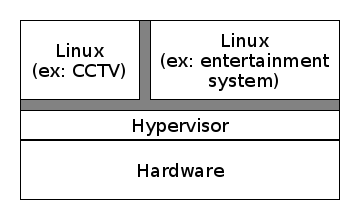
\includegraphics[height=4cm]{figures/figure-hypervisor-simple.png}
	\centering
	\caption{Two Linux on top of an hypervisor. They run isolated from each other and from the hypervisor.}
	\label{figure-hypervisor-simple}
\end{figure}

Previous work in the \acrshort{prosper} project achieved to formally verify a simple separation kernel \cite{noauthor_prosper:_nodate-1,dam_formal_2013}, which later resulted into an implementation of a working hypervisor. Then, they achieved to run both Linux and \gls{FreeRTOS} on top of it. Finally, they formally verified memory isolation for virtualized applications \cite{nemati_trustworthy_2015}. Nowadays, among other projects, the PROSPER team is working on device virtualization, giving access to hardware devices to virtualized applications. \gls{NIC} devices are an interesting example, which enable network communication and give the ability to communicate through the Internet.

A formal model of a \gls{NIC} device has been produced, on which some security theorems have been proved \cite{haglund_formal_2016}.
Indeed, NIC devices are directly connected to the Internet and use \gls{DMA} controllers (cf. Section \ref{dma-mem-sharing}) to access the main memory. Then, rogue virtualized applications could use misconfigured NIC in order to gain access to private information contained in the main memory or even take control of the system. \cite{haglund_formal_2016} showed how to enforce configuration on the NIC in order to prevent rogue behaviors.

These theorems can be seen as high-level proofs relying on a layer of lower-level lemmas (cf. Figure \ref{fringe}). This layer provides an abstraction over the raw formal model. This is illustrated in the left-hand side of Figure \ref{hol-v-bir-nic-model-simple}.

\begin{figure}[ht]
	\includegraphics[height=6cm]{figures/hol-v-bir-nic-model-simple.png}
	\centering
	\caption{HOL4 vs. BIR NIC models. The left hand side already exists. This project consists in the dashed elements. The dotted lines represent the work done during this project.}
	\label{hol-v-bir-nic-model-simple}
\end{figure}

The team is now developing a new platform for performing binary analysis in HOL4, an interactive theorem prover, named \gls{holba} \cite{noauthor_holba_2019}. This platform is based on two papers written in the team. The first one introduces sound \gls{transpilation} from binary to machine-independent code \footnotemark \cite{metere_sound_2017}. The second paper, ``TrABin: Trustworthy Analyses of Binaries'' \cite{lindner_trabin:_2019}, lays the foundations of the \gls{holba} platform: it formally models \gls{BIR}, introduces various supporting tools, implements two \gls{proof-producing} \glspl{transpiler} (ARMv8 and Cortex-M0), named lifters, and a proof-producing weakest precondition generator for loop-free programs.

\footnotetext{The machine-independent language used in \cite{metere_sound_2017} is an implementation of \gls{bap}'s BIL \cite{noauthor_binary_2019}. This implementation will evolve later in \cite{lindner_trabin:_2019} into BIR that HolBA uses today.}

While this kind of \glspl{transpiler} and weakest precondition tools already exist \footnote{See related discussion in \cite{lindner_trabin:_2019}.}, the novelty in this work is that the transpiler is proof-producing, i.e. it produces a formal proof that both binary representations are equivalent, under the simulation theory, with respect to the \gls{ISA} model \footnote{Several models of different ARM \gls{ISA} have been realized in multiple research institutions, such as ARMv3, ARMv4, ARMv7 \cite{noauthor_canonical_2019, hutchison_trustworthy_2010} and very recently ARMv8 \cite{armstrong_isa_2019}.}. With this method, you no longer need to trust the transpiler. Figure \ref{holba-overview} gives an overview of the HolBA platform.

\begin{figure}[ht]
	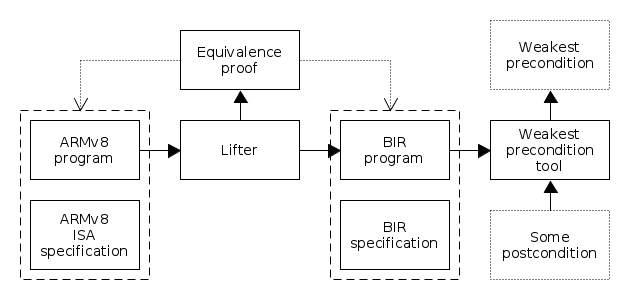
\includegraphics[height=5cm]{figures/holba-overview.png}
	\centering
	\caption{The HolBA platform. The lifter generates a BIR program and an equivalence proof from an ARMv8 program. The equivalence proof establishes a simulation property between the ARMv8 binary program and the generated BIR binary program, showing that they have the same behavior with respect to the ARMv8 \gls{ISA} specification and the BIR specification. HolBA also supports the Cortex-M0 ISA.}
	\label{holba-overview}
\end{figure}

The idea of this work is to translate the formal \gls{NIC} model of \cite{haglund_formal_2016} using \gls{BIR}, then use HolBA's proof-producing weakest precondition tool to prove the same lower-level lemmas than the formal model. With all the lemmas proved, the security properties are implied. Figure \ref{hol-v-bir-nic-model-simple} gives an overview of this idea: using the proof-producing weakest precondition tool to bind together a newly written BIR NIC model and the work done on the formal model.

\section{Intended readers}

In this thesis, formal verification is the central topic. The thesis explores how to model a hardware device using a binary analysis platform and describes some formal verification techniques. A reader interested in this topic may find the results useful for further work. A casual reader will be presented with a light introduction to the concepts that are essential in order to understand the problem that this thesis aims to explore. Those concepts should also be useful in order to understand software verification in general. For a more coherent reading, the concepts are introduced throughout the document. However, the reader is expected to have a background in Computer Science in general, and knowledge in formal verification will make the thesis easier to digest.

\section{Thesis objective}

The primary goal of this thesis project is to explore verification techniques in order to automate parts, if not all, of the verification process of hardware devices using the HolBA platform. The formal \gls{NIC} model of \cite{haglund_formal_2016} is used as working example.

The ultimate goal would be to obtain a fully automatic pipeline for performing such verifications. However, it is evident that this goal isn't reachable in such a small amount of time, or even at all. Thus, this thesis focuses instead on exploring what toolkit is needed in order to facilitate this work.

\section{Delimitations}

This work being about exploration of techniques towards automation of verification techniques, instead of being about producing an actual complete proof of a hardware device, some implementations have not been completed in order to save time to explore in more areas. Additionally, this work mainly concerns the HolBA platform that is developed in the team where this thesis took place.

\section{Choice of methodology}

This work has been carried out step-by-step toward an ideal goal, i.e. re-establishing all the security properties. On the road, needs have been identified and tools have been implemented in order to tackle them. This approach made sense in this particular work because the needs were not known in advance, and therefore needed to be identified. This thesis presents the steps taken during this work, the motivations of each tool that have been implemented, and discusses their limitations and future work in the conclusion.

\chapter{Related work} \label{related-work}
\vspace{-1cm}
\textit{This chapter will present the related work in the domain of secure execution platforms and binary analysis. After briefly introducing memory sharing between \gls{CPU} and devices, it will explain the need for secure execution platforms, present existing binary analysis platforms and explain the novelty of \gls{holba}, the platform used in this work.}

\section{Memory sharing between CPU and devices} \label{dma-mem-sharing}

Figure \ref{cpu-memory-schema} represents how the \gls{CPU} and devices can share the main memory using \acrfull{DMA}. To read from/write to the main memory, the CPU passes through the \gls{MMU}, which is responsible for virtual/physical address translation. In a nutshell, when an operating system is used, every process uses addresses mapped in a virtual address space. The virtual address spaces are set up by the operating system. When a process wants to access the memory, e.g. for reading its value, the request goes through the MMU that translates the virtual address to a concrete physical address. Then, processes run in apparent isolation and can not access other processes memory without permission from the operating system. This architecture provides strong security guarantees, providing the soudness of the operating system (i.e. absence of bugs).

Similarly, devices can directly access the main memory using DMA. This technique enables to offload the CPU from copying each byte of memory by setting the DMA controller to do so. DMA controllers also give devices direct access to the main memory. While fast and convenient, DMA creates a whole new range of vulnerabilities. Indeed, if misconfigured, DMA controllers can give complete access to the main memory to devices, like kernel private memory, page table or executable memory \cite{schwarz_formal_2014}.

\begin{figure}[!t]
	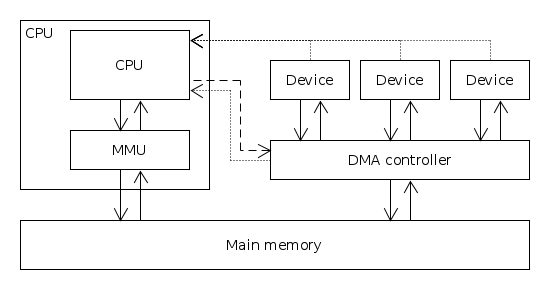
\includegraphics[height=5cm]{figures/cpu-memory-schema.png}
	\centering
	\caption{CPU schema from a memory point of view. The dashed line between the CPU and the DMA controller represent the capability of the CPU to send commands to the DMA controller through register writes. Dotted lines to the CPU represent the ability to raise interrupts. This schema doesn't represent caches.}
	\label{cpu-memory-schema}
\end{figure}

\section{The necessity of secure execution platforms}

The \acrshort{prosper} project isn't the only project focused on high-security execution platforms. Platforms such as seL4, Microsoft Hyper-V and INTEGRITY Multivisor are examples of platforms already used in production and providing strong security properties.

\paragraph{seL4} is a recent L4-based microkernel created in 2006 with the goal to produce a completely formally verified implementation of an L4 microkernel. This has been achieved in 2009 \cite{klein_sel4:_2009}. At this time, seL4 consisted of \num{8700} lines of C code and \num{600} lines of assembler. The implementation of seL4 has been formally proved from its abstract specification down to its C implementation. Later, the validity of the generated assembly code has been proved, removing the need of trusting the compiler \cite{noauthor_what_nodate}.

\paragraph{Microsoft Hyper-V} is Microsoft's hypervisor, widely used today within the Microsoft Azure cloud platform. It has been released in 2008. Hyper-V is a huge codebase, as we can read on VCC's website \footnote{\url{https://www.microsoft.com/en-us/research/project/vcc-a-verifier-for-concurrent-c/}}: ``Hyper-V consists of about 60 thousand lines of operating system-level C and x64 assembly code, it is therefore not a trivial target''. Microsoft has put a lot of work in formal verification\footnotemark of Hyper-V down to machine code \cite{leinenbach_verifying_2009}. However, they don't appear to include device drivers in their formal verification.

\footnotetext{Microsoft has several formal verification projects, many of which are freely available for non-commercial use: \url{https://github.com/Microsoft?q=verifier}}

\paragraph{INTEGRITY Multivisor} is a commercial real-time operating system and hypervisor developed by Green Hills Software. Although not much information seems to be publicly available, Green Hills Software has done considerable formal verification work \cite{richards_modeling_2010}. Multivisor has several certifications, including, for example, ISO 26262 ASIL D automotive electronics, NSA-certified secure mobile phones or FAA DO-178B Level A-certified avionics controlling life-critical functions on passenger and military aircraft \footnote{\url{https://ghs.com/products/rtos/integrity_virtualization.html}}.

\paragraph{MINIX 3} is an operating system whose design is focused on high reliability and security. It is based on a tiny microkernel with the least responsibilities possible, and the rest of the operating system is running as a number of isolated user processes. MINIX 3 has not been formally verified, but intends to provide strong security guarantees by design.

\section{Binary analysis platforms}

For this project, we will use the \gls{holba} platform. However, several other binary analysis platforms have been created for various purposes, such as formal verification or static analysis. A common characteristic of these platforms is to use an \gls{IR}. IRs are designed to be simpler to use for each platforms' end purpose. As an example, the HolBA platform has BIR as its intermediate representation.

\paragraph{Microsoft Boogie} is Microsoft's intermediate verification language. Boogie is the IR for multiple Microsoft tools, including VCC. Boogie as a tool can infer some invariants on the given Boogie program and then generate verification conditions that are passed to an SMT solver \footnote{\url{https://www.microsoft.com/en-us/research/project/boogie-an-intermediate-verification-language/}}.

\paragraph{Valgrind} is a framework for building program supervision tools, such as memory checkers, cache profilers or data-race detectors \cite{nethercote_valgrind:_2003}. As its core, Valgrind is a JIT x86-to-x86 compiler, translating binary programs into its IR called UCode. Then, \textit{skins}---tools built using the Valgrind framework---are free to work with the IR in order to perform their analysis.

\paragraph{LLVM} is a compiler infrastructure which supports a unique multi-stage optimization system \cite{lattner_llvm:_2002}. LLVM is built around its \gls{IR}, LLVM Virtual Instruction Set, which can be described as a strict RISC architecture with high-level type information. This IR made LLVM successful because it is a pragmatic IR suitable for optimizations at multiple stages (link-, post-link, and run-time) and supporting a wide variety of transformations. Leveraging this IR, an ecosystem grew around LLVM, providing tools such as symbolic execution (LLVM KLEE), benchmarking environments or static and dynamic analyzers.

\paragraph{Mayhem} is a system for automatically finding exploitable bugs in binary programs and generating working exploits as proof of the discovered vulnerabilities \cite{cha_unleashing_2012}. It leverages BAP, the Binary Analysis Platform from Carnegie Mellon University (CMU BAP) \cite{brumley_bap:_2011}, as its IR. It proceeds by first JIT-ing each instruction to the BAP intermediate language (IL) and then performing a custom symbolic execution.

There are several other tools, platforms, and frameworks, such as \gls{bap} \cite{noauthor_binary_2019} or Angr. An interesting note though is that BIR's design is based upon CMU BAP's intermediate language.

The novelty introduced in HolBA is that proofs are performed, directly on the generated assembly code, not at the source code level. Therefore, proofs can be performed on programs without needing their source code, and regardless on the programming language used as long as it can be compiled in assembly code in an \gls{ISA} supported by the platform.


\chapter{Overview of the formal verification of the NIC device} \label{chapter-overview-nic}
\vspace{-1cm}
\textit{This chapter will introduce the formal verification of \cite{haglund_formal_2016} that will serve as a guideline throughout this work. It will first introduce Interactive Theorem Proving and formal verification in HOL4, then give a brief overview of the formal NIC model and its proof.}

\section{Interactive Theorem Proving and HOL4} \label{hol4-presentation}

Interactive theorem provers are software producing formal proofs, in an
interactive fashion, i.e. a human can step through the proof interactively while the proof assistant provides some automation (like rewriting of terms, arithmetic evaluation, integration with external tools like SMT solvers, \dots). Coq, HOL4 or Isabelle are such tools.

HOL4 \cite{noauthor_hol_nodate} stands for Higher-Order Logic. It is a programming environment deeply embedded into the \gls{SML} programming language enabling to prove theorems and write \gls{proof-producing} programs. Since its first version in 1988, HOL has been focused on hardware verification and has been successfully used in this domain, as shows its \texttt{examples/} directory \cite{noauthor_canonical_2019}.

HOL4 is built around a very small kernel: 3 axioms, 10 inference rules, two predefined constants, and two types \cite{tuerk_interactive_nodate} \footnotemark. A theorem can only be built using this core, every other higher-level theory must be built from lower-level ones. Furthermore, the kernel consists of very few lines of code, leaving less space for bugs. Hence, for this reason, the trust needed is far inferior to standard systems.

\footnotetext{This is true for the Hol Light Kernel, however, the HOL4 kernel has slightly deviated from this simplicity for historical and performance reasons.}

A proof is a demonstration that a proposition is true. In HOL4, proofs are held inside \textit{theorems}, stating that its proposition \textit{can be proved}. This theorem prover offers two ways of building proofs: in a forward and a backward style. A forward proof derives new theorems using axioms and inference rules: one starts with the building blocks and describes how to combine them. Backwards proofs start instead from the goal to be proved and progress in the proof towards obtaining axioms or known theorems. HOL4 puts emphasis on backward proofs, using tactics. Since every theorem is inferred from the small kernel, forward proofs must be ultimately used. Therefore, automation and tactics are written as forward proofs, and used in backward proofs.

To illustrate the idea of forward and backward proofs, and tactics, let's prove the same proposition using the two approaches (since forward proofs quickly requires wide knowledge of HOL4, the following theorem is a simple contrived example).

\begin{theorem}
\begin{equation}
    \forall p.~p \implies p
    \label{hol4-simple-eq-for-proof}
\end{equation}
\end{theorem}

{
\renewcommand*{\proofname}{Forward proof}
\begin{proof}
Let's start with a free variable $p$ of boolean type. Then, assuming $p$ we have that $p$ is true (assumptions are written in square brackets):
$$[p]~~p$$
Let's discharge the hypothesis. We obtain:
$$p \implies p$$
Finally, we generalize this theorem over all boolean variable, concluding the proof.
\end{proof}
}

In this proof, the discharge and generalize operations are inference rules, available as base lemmas already proved from the kernel. In the following backward proof, emphasised words in squared brackets are tactics corresponding to the written explanation of the sentence.

{{
\renewcommand*{\proofname}{Backward proof}
\begin{proof}
Universal quantifier can be added to free variables, so let's remove them [\textit{GEN\_TAC}]. The goal becomes:
$$p \implies p$$
Let's discharge the implication into an assumption [\textit{DISCH\_TAC}]. The goal becomes:
$$[p]~~p$$
Finally, we can use the assumptions in order to prove the goal [\textit{ASM\_REWRITE\_TAC}].
\end{proof}
}

In this contrived example, the two proofs are exact opposite of each other. In more complex proofs, it is often infeasible to use forward proofs because it requires to many operations and doesn't offer automation.

In HOL4, a theory is a coherent set of theorems and definitions. Theories are written in \gls{SML} script files, then compiled into a theory. A definition is the equivalent concept than when using the $\eqdef$ symbol: a symbol or function is defined to be a synonym of a more complex formula.

\section{Overview of the formal NIC model} \label{overview-nic-model}

% \todo{This part is a bit dense. I do not know how much is it clear for a reader that has no previous knowledge about the NIC}

The formal NIC model of \cite{haglund_formal_2016} has been designed from reading the hardware specification of the device because no model nor device driver is freely available.

The NIC model is designed as a transition system with four types of transitions: register read, register write, autonomous, and memory read request reply transitions \footnotemark. They are described by four functions which constitute its public interface: \texttt{read\_nic\_register}, \texttt{write\_nic\_register}, \texttt{nic\_transition\_autonomous} and \texttt{memory\_read\_reply}. Each of these functions update the given NIC state, simulating the real behavior of the NIC. To make the model sound, the state is marked \textit{dead} if the model is asked to describe any transition or operation that is not described by the specification. Dead states represent undefined states and cannot be left with further transitions.

\footnotetext{We will focus on autonomous transitions in this document, so the other types of transitions are not further described.}

The model is composed of five finite state automata describing the inner transitions of the whole system, each automata describing a part of the NIC. The five automata are initialisation, transmission, transmission teardown, reception and reception teardown. The function \texttt{nic\_execute} performs one autonomous step of one of the five automata. The automaton that takes a step is decided by a scheduler, depending on the NIC inner state. If more than one automaton are in a ready state, their order is not deterministic \footnote{To reason about non-determinism, the notion of oracles has been introduced in \cite{haglund_formal_2016}. To put it simply, an oracle can be seen as a list of steps to perform, but where each element of the list is undefined. As we will not directly reason about the oracle, we will not explain how this works in more details. The reader can read a thorough explanation in \cite{haglund_formal_2016}.}. Each finite state automata is defined as a set of transitions working on NIC states. Each transition takes a NIC state and returns an updated one, possibly dead.

Being designed as a transition system, each of the four functions described earlier is loop-free, aspect that is crucial in order to apply contract-based verification as described in Section \ref{contract-based-verif}. Each transition is implemented as a HOL4 function using exclusively \textbf{if-then-else} and state modification statements. There is no recursive definition. Hence, every function can be seen as some kind of decision tree in which some of the nodes ``mutate'' the state. % This idea will be refined later on in Section \ref{visualizing-cfg}.

The five automata are of different complexity, as shown in Table \ref{stats_complexity_formal_nic_model}, with the initialization automaton having only 4 transitions of which only one is autonomous, and the reception automaton being the most complex with 20 transitions. Calling the \texttt{nic\_transition\_autonomous} function makes one of the automata take an autonomous step. Non autonomous transitions are performed by the three other functions.

\begin{table}[ht!]
    \centering
    \begin{tabular}{ | l | c | c | c | }
        \hline
        Automaton & \# of (autonomous) transitions & LoC (w/o comments)\\
        \hline
        Initialization & 4 (1) & 21\\
        Transmission & 7 (5) & 182\\
        Transmission teardown & 5 (4) & 67\\
        Reception & 20 (20) & 280\\
        Reception teardown & 7 (6) & 93\\
        \hline
    \end{tabular}
    \caption{Statistics on each of the automata in the formal NIC model.}
    \label{stats_complexity_formal_nic_model}
\end{table}

The NIC state is defined as a nested \textit{datatype}---a record \footnote{Records in HOL4 are analogous to structures in imperative languages.} of records of words, booleans and enumerations. However, there is one exception: the NIC works on a memory data structure, called \texttt{CPPI\_RAM}, which is represented in the formal model as a function from addresses to values.

The structure of the implementation of \texttt{read\_nic\_register} and \texttt{write\_nic\_register} is similar to the implementation of \texttt{nic\_transition\_autonomous} in terms of the statements they use. \texttt{memory\_read\_reply} is implemented as a non autonomous transition of the transmission automaton.

\section{Overview of the formal proof of the NIC model} \label{overview-nic-proof}

It has been formally proved with HOL4 that with \gls{prosper}'s hypervisor, augmented with a monitor and in the presence of a \gls{NIC}, only signed Linux code is executed. This security policy has been defined as an invariant of the NIC state, then the proof consists of verifying that each transition of the NIC transition system preserves the invariant. This invariant states that the NIC isn't in an undefined state (represented by the dead state), that the transmission and reception queue are well-behaving (non-overlapping, finite) and that the NIC is in a valid state (restrict the values of the NIC state variables to valid configurations). This invariant is stated as a conjunction of the invariants of each automaton plus a not-dead conjunct:

\begin{equation}
    I_{NIC} \eqdef \neg NIC.dead~\land~I_{init}~\land~I_{tx}~\land~I_{td}~\land~I_{rx}~\land~I_{rd}
    \label{final-nic-proof-invariant}
\end{equation}

Each sub-invariant is proved individually on its respective part of the NIC model, then they are composed together in order to form the final one in Equation \ref{final-nic-proof-invariant}.

The majority of the lemmas are phrased in the same way, that we shall see in Chapter \ref{contract-based-verif} correspond to the equation of Hoare Triples:

\begin{equation}
  I~nic \land nic' = transition~nic \implies I~nic'
  \label{nic-typical-lemma}
\end{equation}

\subsection{Visualizing proof dependencies}

The model of the NIC consists of \num{1500} lines of HOL4 code and required around three man-months of work. The NIC invariant consists of \num{650} lines of HOL4 code and the proof consists of approximately \num{55000} lines of HOL4 code including comments. Identifying the invariant and implementing the proof in HOL4 required around one man-year of work \cite{haglund_trustworthy_nodate}.

\begin{figure}[tb]
	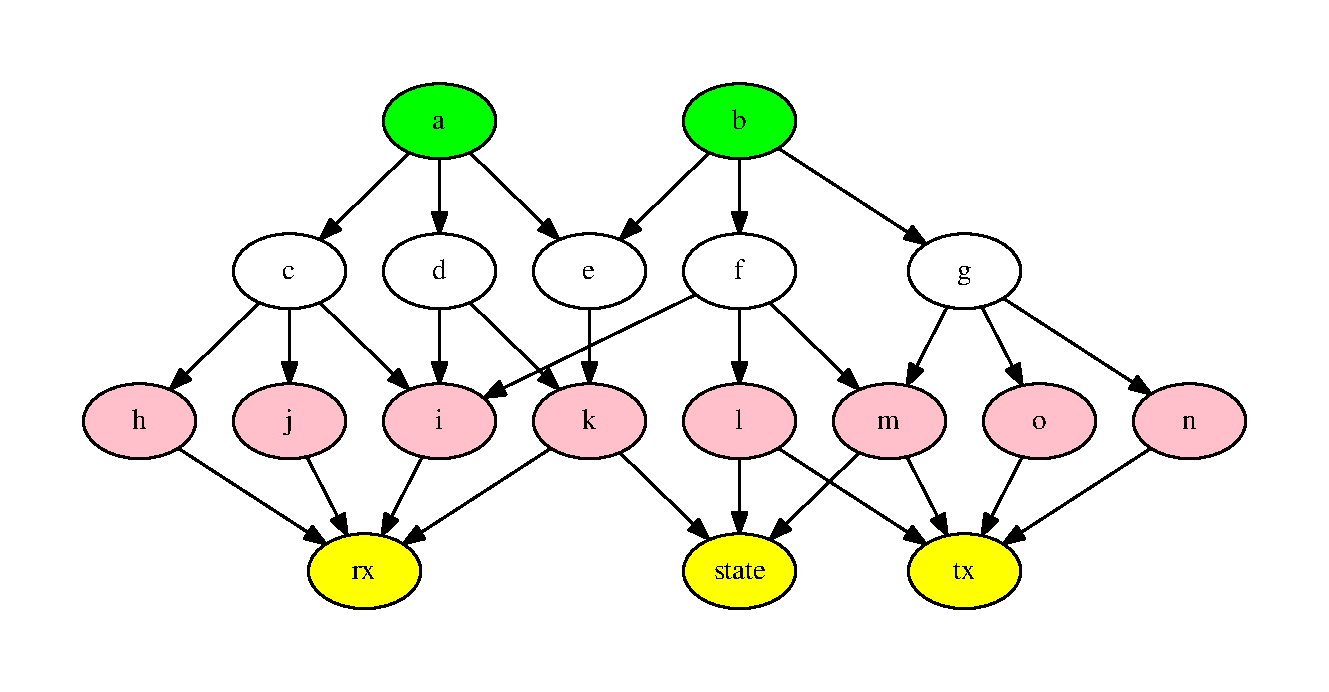
\includegraphics[height=5cm]{figures/fringe.pdf}
	\centering
	\caption{Representation of the fringe on an ideally shaped formal proof. Green nodes represent the security theorems, pink nodes the fringe that interests us (the ``base lemmas'') and the yellow ones the formal model. A directed edge from $A$ to $B$ means that $A$ depends on $B$.}
	\label{fringe}
\end{figure}

The proof is substantially large: it is composed of a multitude of lemmas spread out in multiple layers. The ideal objective of this work is to prove again the base lemmas on a different but equivalent BIR program. Therefore, we need to identify the relevant lemmas to be replaced. The proof is divided into two major parts, reception and transmission, and lemmas are scattered across a few files, each file being for a different part or abstraction level. Optimally, identifying the fringe of the dependency graph of the lemmas and theorems would give exactly the set of lemmas that all the other lemmas and theorems rely on, and therefore the smallest set of lemmas that are enough to prove in order to imply the security properties already proved in \cite{haglund_trustworthy_nodate} by using the existing proofs. Figure \ref{fringe} gives a visual representation of this idea.

As an attempt to visualize this fringe, we developed a tool, called DepGraph \footnote{DepGraph's design is presented in Appendix \ref{appendix_depgraph}.}, that can extract the dependency structure of HOL4 proofs in the form of a dependency graph. DepGraph features two frontends that can extract dependencies between HOL4 theories (i.e. autogenerated \gls{SML} files containing proofs of lemmas and theorems), and between definitions, theorems, and lemmas. Figure \ref{depgraph-nic-tx-files} shows the dependencies between theories about the transmission part of the NIC proof, and Figure \ref{depgraph-nic-tx-thms} shows the dependencies between definitions, theorems and lemmas of the same part of the proof. However, as can be seen on Figures \ref{depgraph-nic-tx-files} and \ref{depgraph-nic-tx-thms}, this tool presents some critical shortcomings:

\begin{itemize}
	\item The theory dependencies frontend uses files generated by Holmake, the HOL4 compile system, in order to get the dependencies between theories. However, those files don't really represent dependencies but the files to be loaded before this script can be loaded, in a recursive fashion. Therefore, they represent the transitive reduction of the dependency graph. Figure \ref{transitive-reduction} presents transitive reduction. Because of this fact, precious knowledge is lost and cannot be recovered by using this method: edges representing direct dependencies can be removed if the remaining edges still account for this dependency. Therefore, we are still able to tell which nodes depend on some node $n$, but we cannot identify the aforementioned fringe. In order to solve this problem, different approaches exist, such as implementing a simplified SML parser that looks only at dependencies, or injecting code inside the dependency resolution of an existing SML compiler. However, this would involve too much work that isn't the direct focus of this thesis.
	\item The definition, theorem and lemma dependencies frontend uses word-based heuristics in order to extract dependencies, and is as such not quite reliable and cannot give any guarantee. As above, there exist similar solutions in order to get multiple levels of guarantees, such as implementing a SML parser or injecting code inside HOL4 theory and definitions handling, but this would also require too much work. Destructuring HOL4 theories does not work because of how HOL4 has been designed, i.e. no trace is kept on disk about how to prove a given saved theorem, except of course with the corresponding script file. Moreover, such dependency graphs become quickly big, making them unusable in practice, and some additional work would be needed in order to represent them in a convenient way. Therefore, as above, no further work has been put into this frontend.
\end{itemize}

\begin{figure}[p]
	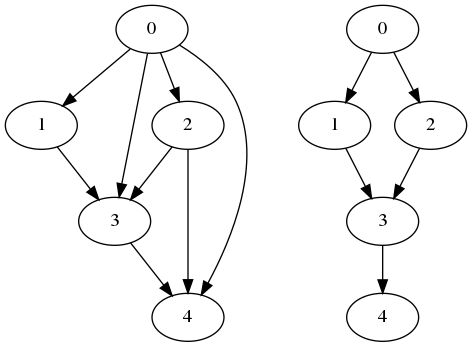
\includegraphics[height=5cm]{figures/transitive-reduction.png}
	\centering
	\caption{The right-hand side graph represent the transitive reduction of the left-hand side graph. Edges $(0 \rightarrow 3)$, $(0 \rightarrow 4)$ and $(2 \rightarrow 4)$ have been deleted because the transitive dependency relationship is preserved in the remaining edges. For example, the dependency $(0 \rightarrow 3)$ is represented in paths $(0 \rightarrow 1  \rightarrow 3)$ and $(0 \rightarrow 2 \rightarrow 3)$.}
	\label{transitive-reduction}
\end{figure}

\begin{figure}[p]
%python3 -m depgraph \
%    --log=debug \
%    --hol4 /NOBACKUP/tholac/nic_model/invariant/tx \
%    --exclude-dependencies "HOL4/" \
%    --highlight-dependents-of txTheory yellow \
%    --highlight-leafs red \
%    --as-dot --dot-horizontal \
%    | dot -Tpdf > /tmp/depgraph/depgraph-nic-tx-files.pdf
	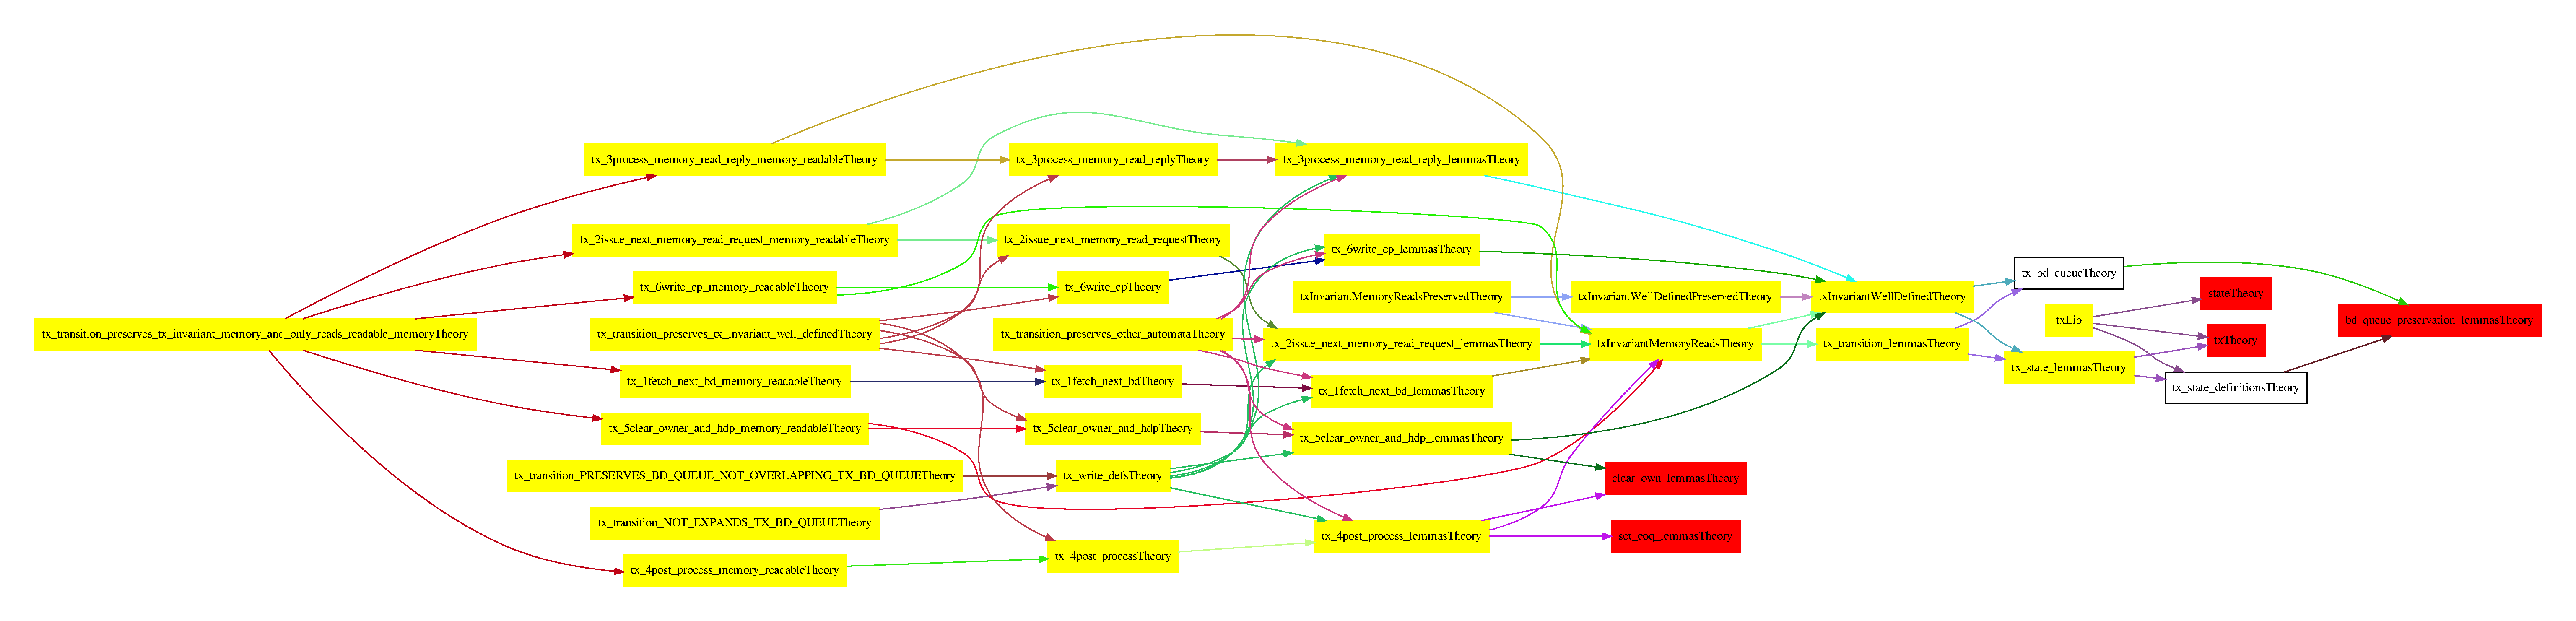
\includegraphics[width=\textwidth]{figures/depgraph-nic-tx-files.pdf}
	\centering
	\caption{Dependency graph between theories about the transmission part of the formal NIC proof. An edge from a node $A$ to a node $B$ means that $A$ depends on $B$. On this figure, edges are directed from left to right. Therefore, on this figure, higher-level files are on the left and lower-level ones on the right. Yellow nodes represent theories that depend on \textit{txTheory}, i.e. the theory describing the transmission automaton presented in Section \ref{overview-nic-model}. Red nodes represent the leaves of the dependency graph, i.e. files without dependencies. Each node's edges are of different colors.}
	\label{depgraph-nic-tx-files}
\end{figure}

\begin{figure}[p]
%python3 -m depgraph \
%    --log=debug \
%    --hol4-thms /NOBACKUP/tholac/nic_model /NOBACKUP/tholac/nic_model/invariant/tx \
%    --highlight-leafs red \
%    --transitive-reduction \
%    --as-dot --dot-horizontal \
%    | dot -Tpdf > /tmp/depgraph/depgraph-nic-tx-thms.pdf
	\includegraphics[width=\textwidth]{figures/depgraph-nic-tx-thms.pdf}
	\centering
	\caption{Dependency graph between definitions, theorems, and lemmas of the transmission part of the formal NIC proof. An edge from a node $A$ to a node $B$ means that $A$ depends on $B$. Therefore, on this figure, higher-level files are on the left and lower-level ones on the right. Each node's edges are of different colors. Red nodes represent leaf nodes, i.e. theorems and definitions without dependencies. The red nodes on the left-hand side of the Figure are nodes for which the heuristic failed to capture the dependencies.}
	\label{depgraph-nic-tx-thms}
\end{figure}

\chapter{The BIR NIC model} \label{nic-model}
\vspace{-1cm}
\textit{This chapter compares different approaches of implementing a BIR model that is equivalent to the formal NIC model. After an introduction of BIR, it will present different possible ways of doing this translation and present three approaches. Then, the final BIR model will be introduced along with the new tools that have been implemented in order to build it.}

\section{HolBA's Binary Intermediate Representation (BIR)} \label{bir-presentation}

HolBA's Binary Intermediate Representation (BIR) \cite{lindner_trabin:_2019} is a  machine-independent binary representation. It aims to be simple while still being able to represent all possible binary programs except self-modifying programs. It does so by having a limited syntax---introduced in Table \ref{bir-syntax}---and forbidding implicit side-effects. A statement can only have explicit state changes and can only affect one variable.

\begin{table}[ht]
	\begin{align*}
		prog   & :=~block^{\ast}                                                             \\
		block  & :=~(string~|~integer,~stmt^{\ast},~estmt)                                   \\
		stmt   & :=~\textbf{assign}~(string, exp)~|~\textbf{assert}~(exp)~|~\textbf{assume}~(exp)  \\
        estmt  & :=~\textbf{jmp}~(exp)~|~\textbf{cjmp}~(exp,~exp,~exp)~|~\mathbf{halt}~(exp) \\
		exp    & :=~integer~|~\textbf{var}~string                                            \\
		       & ~~~~|~\textbf{if-then-else}~(exp,~exp,~exp)                                 \\
		       & ~~~~|~\diamond_{u}~exp~|~exp~\diamond_{b}~exp~                              \\
		       & ~~~~|~\textbf{load}~(exp,~exp,~\tau)~|~\textbf{store}~(exp,~exp,~exp,~\tau) 
	\end{align*}
  \caption{BIR's syntax. Valid BIR programs must be well-typed. $integer$s represent bounded N-bit integers. $\diamond_{u}$ and $\diamond_{b}$ represent respectively unary and binary operators. BIR blocks are tuples, with the first element being its label, the second a list of statements and the third the end statement.
  \textbf{assign} is the only statement that can mutate the execution state, and can only affect one variable at a time. \textbf{assert} and \textbf{assume} allow imposing conditions on programs, respectively asserting that an expression is true (or abort otherwise) and assuming that an expression is true. This is useful for analysis. \textbf{jmp} and \textbf{cjmp} allow to control the Control Flow of programs using respectively direct and conditional jumps. \textbf{halt} represents termination of programs.
  BIR syntax contains some other statements that won't be used in this work and that have been omitted. See \cite{lindner_trabin:_2019} for more information.}
	\label{bir-syntax}
\end{table}

This representation allows producing proofs more easily that with classical binary representations, whose design are focused on execution speed rather than offline analysis.

% BIR is implemented as a set of HOL4 data types. Since HOL4 is a theorem prover, definitions are theorems stating formal definitions. As such, it is fully described in terms of both syntax and semantics.
% \todo{This can be rephrased}
% Section \ref{bir-memories-with-smt-solvers} contains a more thorough discussion of the BIR semantics. Section \ref{alice-bob-toy} implements a toy BIR program and presents the concrete BIR syntax.
% This is not very useful at this point, I think.

Among its supporting tools, HolBA features a tool to visualize the \gls{CFG} of BIR programs.

\section{Exploring multiple approaches to translating the formal NIC model}

We considered multiple approaches to translate the formal NIC model to an equivalent BIR program:

\begin{itemize}
    \item \textbf{handwritten BIR program}: The most straightforward way would be to directly write the BIR program by hand by looking at the actual formal model and directly converting it to BIR. This is easily feasible because of the limited set of statement used in the implementation of the NIC model which are all representable in the BIR syntax. However, this does not seem optimal if more than one such translation need to be performed. One remedy of this problem would be to implement a set of tools that facilitate the implementation of device models and reduce the boilerplate. This idea is explored in the following Sections \ref{alice-bob-toy} to \ref{impl-real-model}.
    \item \textbf{lifted C program}: An alternative would be to implement the NIC model in a more convenient higher-level programming language, compile it to assembly code and leverage the existing lifter to generate a BIR program. One advantage of this method is the possibility to use existing frameworks and tools that already exist in other languages, in which the ease of development is higher. However, the gained ease of development is maybe not worth the complexity introduced by those steps. The following Section \ref{c-model} experiments this idea.
    \item \textbf{device model specific \gls{IR}}: This idea rejoins the previous one in the sense that it uses an additional intermediate representation (C in the previous idea) to implement the model, then uses some compiler to generate the BIR program (standard C compiler and HolBA's lifter). This idea would have the advantage that it introduces a new higher-level IR that would be common to possible later other device modelizations. Tools could also be developed for this IR. However, this approach would require to develop a new IR and, if we later want to develop a \gls{proof-producing} lifter (compiler) the implementation would be costly, especially since this language would be more complex. The following Section \ref{flowchart-attempt} tries to use a visual flowchart language as IR. %This idea has not been explored in this work, where we decided to experiment using existing tools: the lifter, BIR, and its supporting tools.
\end{itemize}

\subsection{Using flowcharts as Intermediate Representation} \label{flowchart-attempt}
% essayé flowcharts, simple mais taille grossit très vite, complexe, tedious

As already discussed in the previous Section, the structure of the formal model looks like a tree. Therefore, using flowcharts can be a convenient way to represent such structures. An attempt has been made to design a flowchart representation. Figures \ref{flowchart-scheduler}, \ref{flowchart-tx} and \ref{flowchart-tx_fetch_next_bd} show respectively a preview of the scheduler, transmission automaton and particular transition of this automaton.

\begin{figure}[p]
	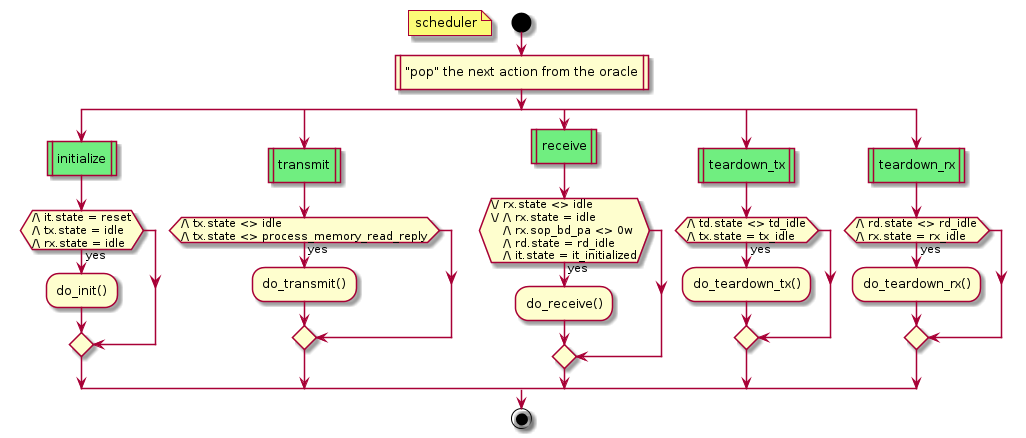
\includegraphics[width=\textwidth]{figures/flowchart-scheduler.png}
	\centering
	\caption{Flowchart of the scheduler of the NIC model. Green nodes represent condition statements, here they represent the value of the popped action from the oracle. The full dot represents the entry point, and the other dot the exit point.}
	\label{flowchart-scheduler}
\end{figure}

\begin{figure}[p]
	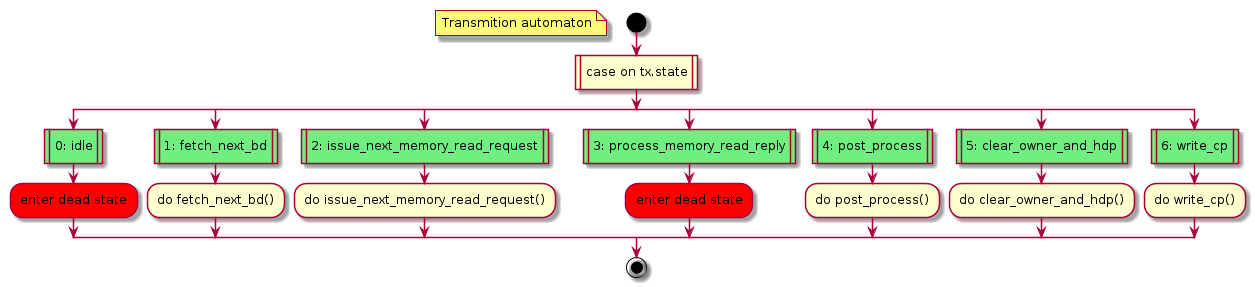
\includegraphics[width=\textwidth]{figures/flowchart-tx.png}
	\centering
	\caption{Flowchart of the transmission automaton of the NIC model. Green nodes are similar to the ones of Figure \ref{flowchart-scheduler}. Red nodes represent non-autonomous transitions leading to dead states.}
	\label{flowchart-tx}
\end{figure}

\begin{figure}[p]
	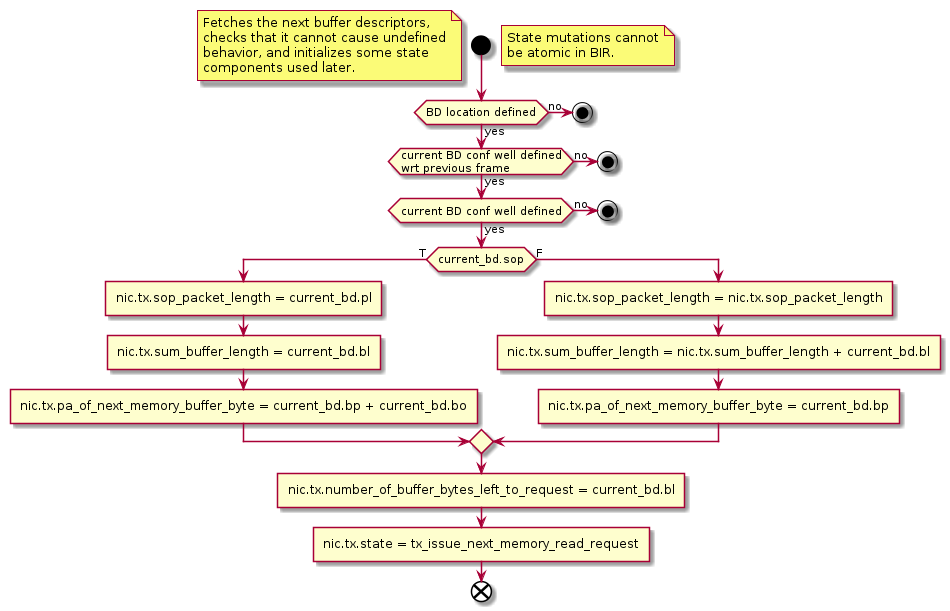
\includegraphics[width=\textwidth]{figures/flowchart-tx_fetch_next_bd.png}
	\centering
	\caption{Flowchart of the \texttt{fetch\_next\_bd} transition of the transmission automaton of the NIC model. The full dot represent the entry point, $\bigotimes$ represents the exit point and the other dots are shorthands to represent dead transitions (the symbols have been changed because of technical limitations of the tool used to draw the diagram).}
	\label{flowchart-tx_fetch_next_bd}
\end{figure}

While this visual representation was useful to get to know the formal NIC model, we encountered several shortcomings:

\begin{itemize}
    \item Flowcharts of each transition rapidly grew in size with the complexity of its formal counterpart. Possible workarounds include the use of nested diagrams, as it is the case of Figure \ref{flowchart-tx_fetch_next_bd} representing one node of Figure \ref{flowchart-tx}, namely \texttt{fetch\_next\_bd}, or usage of shorter ways of representing common patterns, as it is the case for representing dead transitions on Figure \ref{flowchart-tx_fetch_next_bd}.
    \item It is hard to define a coherent visual language able to represent the full set of features needed in order to realize device models. Additionally, this language must be compatible or easily translatable to BIR.
    \item It is hard to design a textual representation of this visual language other than conventional programming languages, so using such representation would require a substantial implementation effort in order to implement all the tools needed to use it. Developing visualization tools for a conventional language appears to be a more reasonable approach than developing a visual language.
\end{itemize}

For those reasons, it has been decided to not go further with this visual representation, and to focus instead on existing tools of the HolBA platform. However, as we shall see in the rest of this thesis, we will explore other visualization tools, and flowcharts will be used as a visual help while designing the model using other methods.

\subsection{Writing the model in C} \label{c-model}

One-to-one translation of the definitions related to the transmission automaton, scheduler, state, and \textit{CPPI\_RAM} of the formal model have been realized in C. This translation has been quite easy to perform and has been completed in roughly one day, and no difficulty arose during this translation. Regarding the NIC state, C has all types needed to represent it. An array has been used to represent the function type of \textit{CPPI\_RAM}. Enumerations have been used in order to represent HOL4 enumerations. While not optimal because of their non-restricted usage allowed by the C language---they can be freely modified as integers without checking their validity in C, while HOL4 and functional languages in general are restrictive and force to use correct values---enumerations are enough if used correctly while being well-aware of those shortcomings.

When studying the compiled assembly code and lifted BIR program, we noticed that all the convenient naming that we can use in the formal or the C model is lost and replaced with abundant usage of the stack. While this is completely normal behaviour for a C compiler, this is not convenient when performing later proofs on the model: we would first need to rename them in the proof using some definitions, and this process would be lengthy and cumbersome (if not automated), resulting in more code than if the model had been directly written in BIR in the first place. This experiment made us realize that writing the model is a rapid operation and that we should rather focus on making the verification step as smooth as possible because it is the most difficult one to perform.

For those reasons, it has been decided to try using BIR directly to write the NIC model. The following Section \ref{alice-bob-toy} presents a first prototype that has been realized in order to visualize the shape of a BIR program representing the NIC model, and identify the tools that would be needed in order to reduce the boilerplate of such implementation in BIR.

\subsection{Implementing a toy BIR model} \label{alice-bob-toy}

Before writing the whole NIC model by hand, we shall identify the structure of the model and develop tools that facilitate its implementation. Using well-designed tools can reduce the boilerplate work of the implementation, helping to focus only on the meaningful content of the implementation, and can also reduce the chance of introducing bugs as the code is factored and mechanically shorter.

We decided to implement a simplified version of the NIC transition system, with only two automata: reception and transmission. In this simplified model, the two automata feature a simple linear transition system, and each of them has one non-autonomous transition, that is performed respectively by two external functions \texttt{memory\_read} and \texttt{memory\_write} that represent memory accesses from the CPU. The function \texttt{autonomous\_step} performs one autonomous transition via the scheduler (Figure \ref{alice-bob-scheduler-oracle}). Figure \ref{alice-bob-automata-overview} gives an overview of the two automata, Figure \ref{alice-bob-entrypoints} shows the role of the three functions and Figure \ref{alice-bob-alice_autonomous_transitions} describes in details the contrived reception automaton. (Flowcharts from the previous Section \ref{flowchart-attempt} have been used in this section in order to facilitate designing the toy model. However, no effort has been made to come up with a coherent and formalized language.)

\begin{figure}[p]
	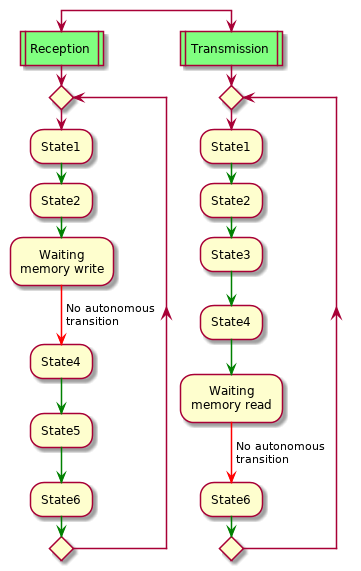
\includegraphics[height=10cm]{figures/alice-bob-automata-overview.png}
	\centering
	\caption{Overview of the two independent automata. Green arrows represent autonomous transitions and red arrows the non-autonomous ones. As in Section \ref{flowchart-attempt}, green nodes represent conditional statements depending on the scheduler's oracle, as shown in Figure \ref{alice-bob-scheduler-oracle}. The states and transitions have no particular meaning in this model.}
	\label{alice-bob-automata-overview}
\end{figure}

\begin{figure}[p]
	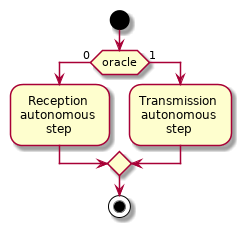
\includegraphics[height=4cm]{figures/alice-bob-scheduler-oracle.png}
	\centering
	\caption{Scheduler of the toy BIR model. We can see how the oracle decides which automaton takes a step. If an automaton is in a state whose transition isn't autonomous, the automaton state is returned unchanged.}
	\label{alice-bob-scheduler-oracle}
\end{figure}

\begin{figure}[p]
	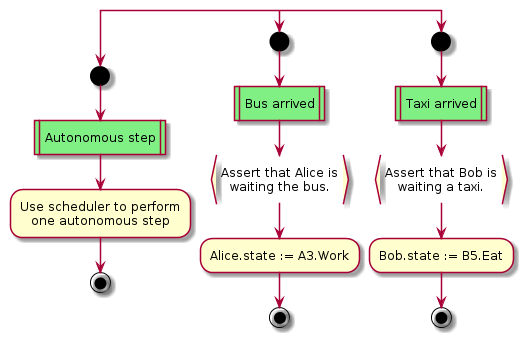
\includegraphics[height=5.5cm]{figures/alice-bob-entrypoints.png}
	\centering
	\caption{The three entrypoints of the toy program: \texttt{autonomous\_step}, \texttt{memory\_read} and \texttt{memory\_write}.}
	\label{alice-bob-entrypoints}
\end{figure}

\begin{figure}[p]
	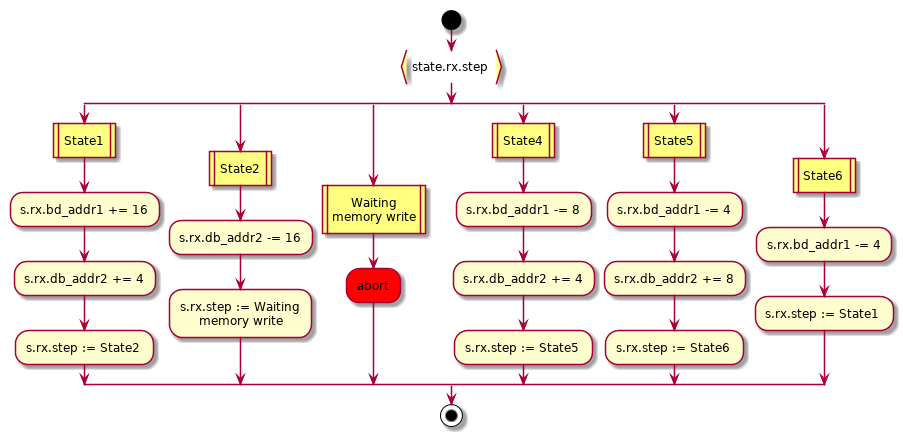
\includegraphics[width=\textwidth]{figures/alice-bob-alice_autonomous_transitions.png}
	\centering
	\caption{The six transitions of the reception automaton. Each transition only updates the state. Conditional statements hasn't been added in this toy model because it already features conditional statements in the scheduler. The third transition is a non-autonomous transition; \texttt{memory\_write} is in charge of updating the reception automaton's state from \textit{WaitingMemoryWrite} to \textit{State4}.}
	\label{alice-bob-alice_autonomous_transitions}
\end{figure}

From the design presented in Figures \ref{alice-bob-automata-overview} to \ref{alice-bob-alice_autonomous_transitions}, writing the BIR program is a repetitive but straightforward step. The resulting BIR program is \num{450} lines of code long. The following issues have been identified:

\begin{itemize}
    \item BIR, as a HOL4 embedded language, is very verbose. Simple operations like additions or assignments require long constructions, as shown in Listing \ref{alice-bob-bir-verbose}. Section \ref{bsl} presents BSL, a less verbose way of writing BIR programs.
\begin{lstlisting}[
    language=Caml,
    backgroundcolor=\color{codebackcolour},
    commentstyle=\color{codegreen},
    keywordstyle=\color{magenta},
    stringstyle=\color{codepurple},
    label=alice-bob-bir-verbose,caption=BIR implementation of one autonomous transition,
    frame=tb,basicstyle=\tiny\ttfamily]
(* RX. State2 *)
<|bb_label := BL_Label "rx_automaton.step.2";
  bb_statements := [
    (* state.rx.bd_addr2 -= 16 *)
    BStmt_Assign (BVar "state.rx.bd_addr2" (BType_Imm Bit32))
      (BExp_BinExp BIExp_Minus
        (BExp_Den (BVar "state.rx.bd_addr2" (BType_Imm Bit32)))
        (BExp_Const (Imm32 16w)));
    (* state.rx.step := 3 *)
    BStmt_Assign (BVar "state.rx.step" (BType_Imm Bit32))
      (BExp_Const (Imm32 3w))
  ];
  bb_last_statement := BStmt_Jmp (BLE_Label (BL_Label "rx_automaton.end"))
|>;
\end{lstlisting}
    \item BIR features only one conditional statement controlling the control flow of a program: conditional jumps. Hence, BIR is not convenient for representing \textbf{if-then-else} statements with more than two branches. Section \ref{impl-real-model} presents some helper functions that have been implemented in order to be able to abstract the raw BIR code and work at a higher level.
\end{itemize}

\subsection{BSL: BIR Simple Language} \label{bsl}

Because of its extreme verbosity, BIR is not a language convenient to manually use. Its primary use has been as an output from the \gls{proof-producing} lifter and as a machine-independent intermediate representation with a very limited feature-set convenient to reason about. A less verbose and more convenient method for producing BIR code is needed in order to open this language to other uses. Therefore, a library has been written that offers the same expressiveness as BIR but with shorter constructs. This library has been kept simple and will serve as the base layer of possible later abstractions. As such, it has been decided that no feature other than pure syntactic construct, such as type inference, would be included. This library has been named BIR Simple Language (BSL) and is implemented in the file \textit{bslSyntax.sml} \footnote{This file has been named in order to follow the HOL4 conventions: \textit{*Syntax.sml} files contain functions that create, destruct and check HOL4 terms. \textit{bslSyntax.sml} is a library for creating only BIR terms, and should, therefore, follow this convention.}.

BSL is composed of a set of functions with short names and a coherent interface. Since this library will be directly included in every \gls{SML} script file in order to avoid usage of the lengthy \texttt{bslSyntax.function\_name} SML construction, we decided to prefix every function with the letter \texttt{b}. As BSL doesn't feature type inference, types must be explicitly given when necessary. For every such function, such as \texttt{bconst}, implementations for every possible type have been added, in addition to general functions taking the size as an argument. Thanks to partial function application in SML, composing functions is easy and scripts can create the set of functions that they need. However, in practice, a BIR program uses a very limited set of types and it is often enough in scripts to statically define the needed set of sized functions (as shown in Listing \ref{bsl-static-funcs}). Finally, BSL has been designed to be fully interoperable with HOL4 terms; it exists for every BIR operation a related BSL function taking a HOL4 term as a parameter, and every BSL function returns a HOL4 term. Therefore, scripts cannot be limited by the restricted feature-set of BSL.

\begin{lstlisting}[
    language=Caml,
    backgroundcolor=\color{codebackcolour},
    commentstyle=\color{codegreen},
    keywordstyle=\color{magenta},
    stringstyle=\color{codepurple},
    label=bsl-static-funcs,caption=Example of prelude of a SML script that defines functions tailor-made to its use. The function \textit{o} is used for function combination.,
    frame=tb,basicstyle=\footnotesize\ttfamily,
    float,floatplacement=H]
val bvarstate = bvarimm32
val bdenstate = (bden o bvarstate)
val bstateval = bconst32
val bjmplabel_str = (bjmp o belabel_str)
\end{lstlisting}

%\subsection{Device model specific BIR helpers} \label{device-bir-helpers}
%% not general enough to be part of BSL, but can be seen as an extension

\subsection{Implementing the real model} \label{impl-real-model}
% model not-complete model (focus on key parts)

From the knowledge gained in the previous section \ref{alice-bob-toy}, a set of helper functions has been implemented, mainly in order to facilitate reasoning about the state machine. Listings \ref{impl-real-tx_state} and \ref{impl-real-tx_bstate_cases} show the SML code respectively used to represent the transmission automaton and to generate the BIR blocks that jump to the right label of the program depending on the current step of the automaton (analogous to a \textit{case} or \textit{switch} construct in higher-level languages).

\begin{lstlisting}[
    language=Caml,
    backgroundcolor=\color{codebackcolour},
    commentstyle=\color{codegreen},
    keywordstyle=\color{magenta},
    stringstyle=\color{codepurple},
    label=impl-real-tx_state,caption={Call to the \texttt{gen\_state\_helpers} function that generates a record containing the list of the states, the list of the autonomous states, a function from state name to state id, a function from state name to boolean telling if the state is autonomous and a function that generates BIR code of the state id from the state name. \texttt{gen\_state\_helpers} takes as parameters the name of the automaton and a list of its states with an id and a boolean telling if the state is autonomous.},
    frame=tb,basicstyle=\footnotesize\ttfamily,
    float,floatplacement=TB]
val tx_state = gen_state_helpers "tx" [
  ("tx1_idle",                          (1, false)),
  ("tx2_fetch_next_bd",                 (2, true)),
  ("tx3_issue_next_memory_read_request",(3, true)),
  ("tx4_process_memory_read_reply",     (4, false)),
  ("tx5_post_process",                  (5, true)),
  ("tx6_clear_owner_and_hdp",           (6, true)),
  ("tx7_write_cp",                      (7, true))
]
\end{lstlisting}
\begin{lstlisting}[
    language=Caml,
    backgroundcolor=\color{codebackcolour},
    commentstyle=\color{codegreen},
    keywordstyle=\color{magenta},
    stringstyle=\color{codepurple},
    label=impl-real-tx_bstate_cases,caption={Autonomous transition jump table used for the transmission automaton. This table uses the names of each state and transition to generate the BIR blocks that will perform the conditional jumps depending on the value of the current transmission state. The parameters of the function are: a tuple of the name of the variable containing the current state, the label of the block to jump to when the current state isn't handled and a function that gives the state number from state name, and a list of jumps, each jump being a tuple of the label of the conditional BIR block, the value of the state that leads to this block and the name of the label to go to.},
    frame=tb,basicstyle=\tiny\ttfamily,
    float,floatplacement=TB]
(* Autonomous transition jump *)
@ bstate_cases ("nic_tx_state", "tx_unknown_state", bstateval_tx) [
  ("tx_try_s1", "tx1_idle",                           "tx_no_autonomous_step_state"),
  ("tx_try_s2", "tx2_fetch_next_bd",                  "tx_s2_entry"),
  ("tx_try_s3", "tx3_issue_next_memory_read_request", "tx_s3_entry"),
  ("tx_try_s4", "tx4_process_memory_read_reply",      "tx_no_autonomous_step_state"),
  ("tx_try_s5", "tx5_post_process",                   "tx_s5_entry"),
  ("tx_try_s6", "tx6_clear_owner_and_hdp",            "tx_s6_entry"),
  ("tx_try_s7", "tx7_write_cp",                       "tx_s7_entry")
]
\end{lstlisting}
%
Because of time constraints, not every transition of the formal NIC model have been implemented in this new model. Instead, we decided to focus on only some transitions in two automata: initialization and transmission. This focus is pragmatic for two reasons: (a) we decided to write the model along with the proof, only the needed transitions for the current proof, in order to grow the model at a reasonable pace and to not clutter it with unneeded features or at the contrary missing critical aspects during the first sketch; (b) as the verification was performed at the same time, we decided to start with easier transitions, but not obvious ones, hence the choice to postpone verification of the more complex reception automaton to later in the work.

When visualizing the \gls{CFG} of the BIR NIC model (Figure \ref{nic-bir-model-cfg}), we notice that it has the shape of a tree, rejoining the idea introduced in Section \ref{overview-nic-model}: each node of the tree is a BIR block, each edge a jump. Since every jump in the NIC model go to a static target, a jump can only have one or two destinations. Hence, nodes can only have one or two outgoing edges. In the model, each node represents either an empty jump block (possibly conditional) or a mutation of the state.

\begin{figure}[p]
	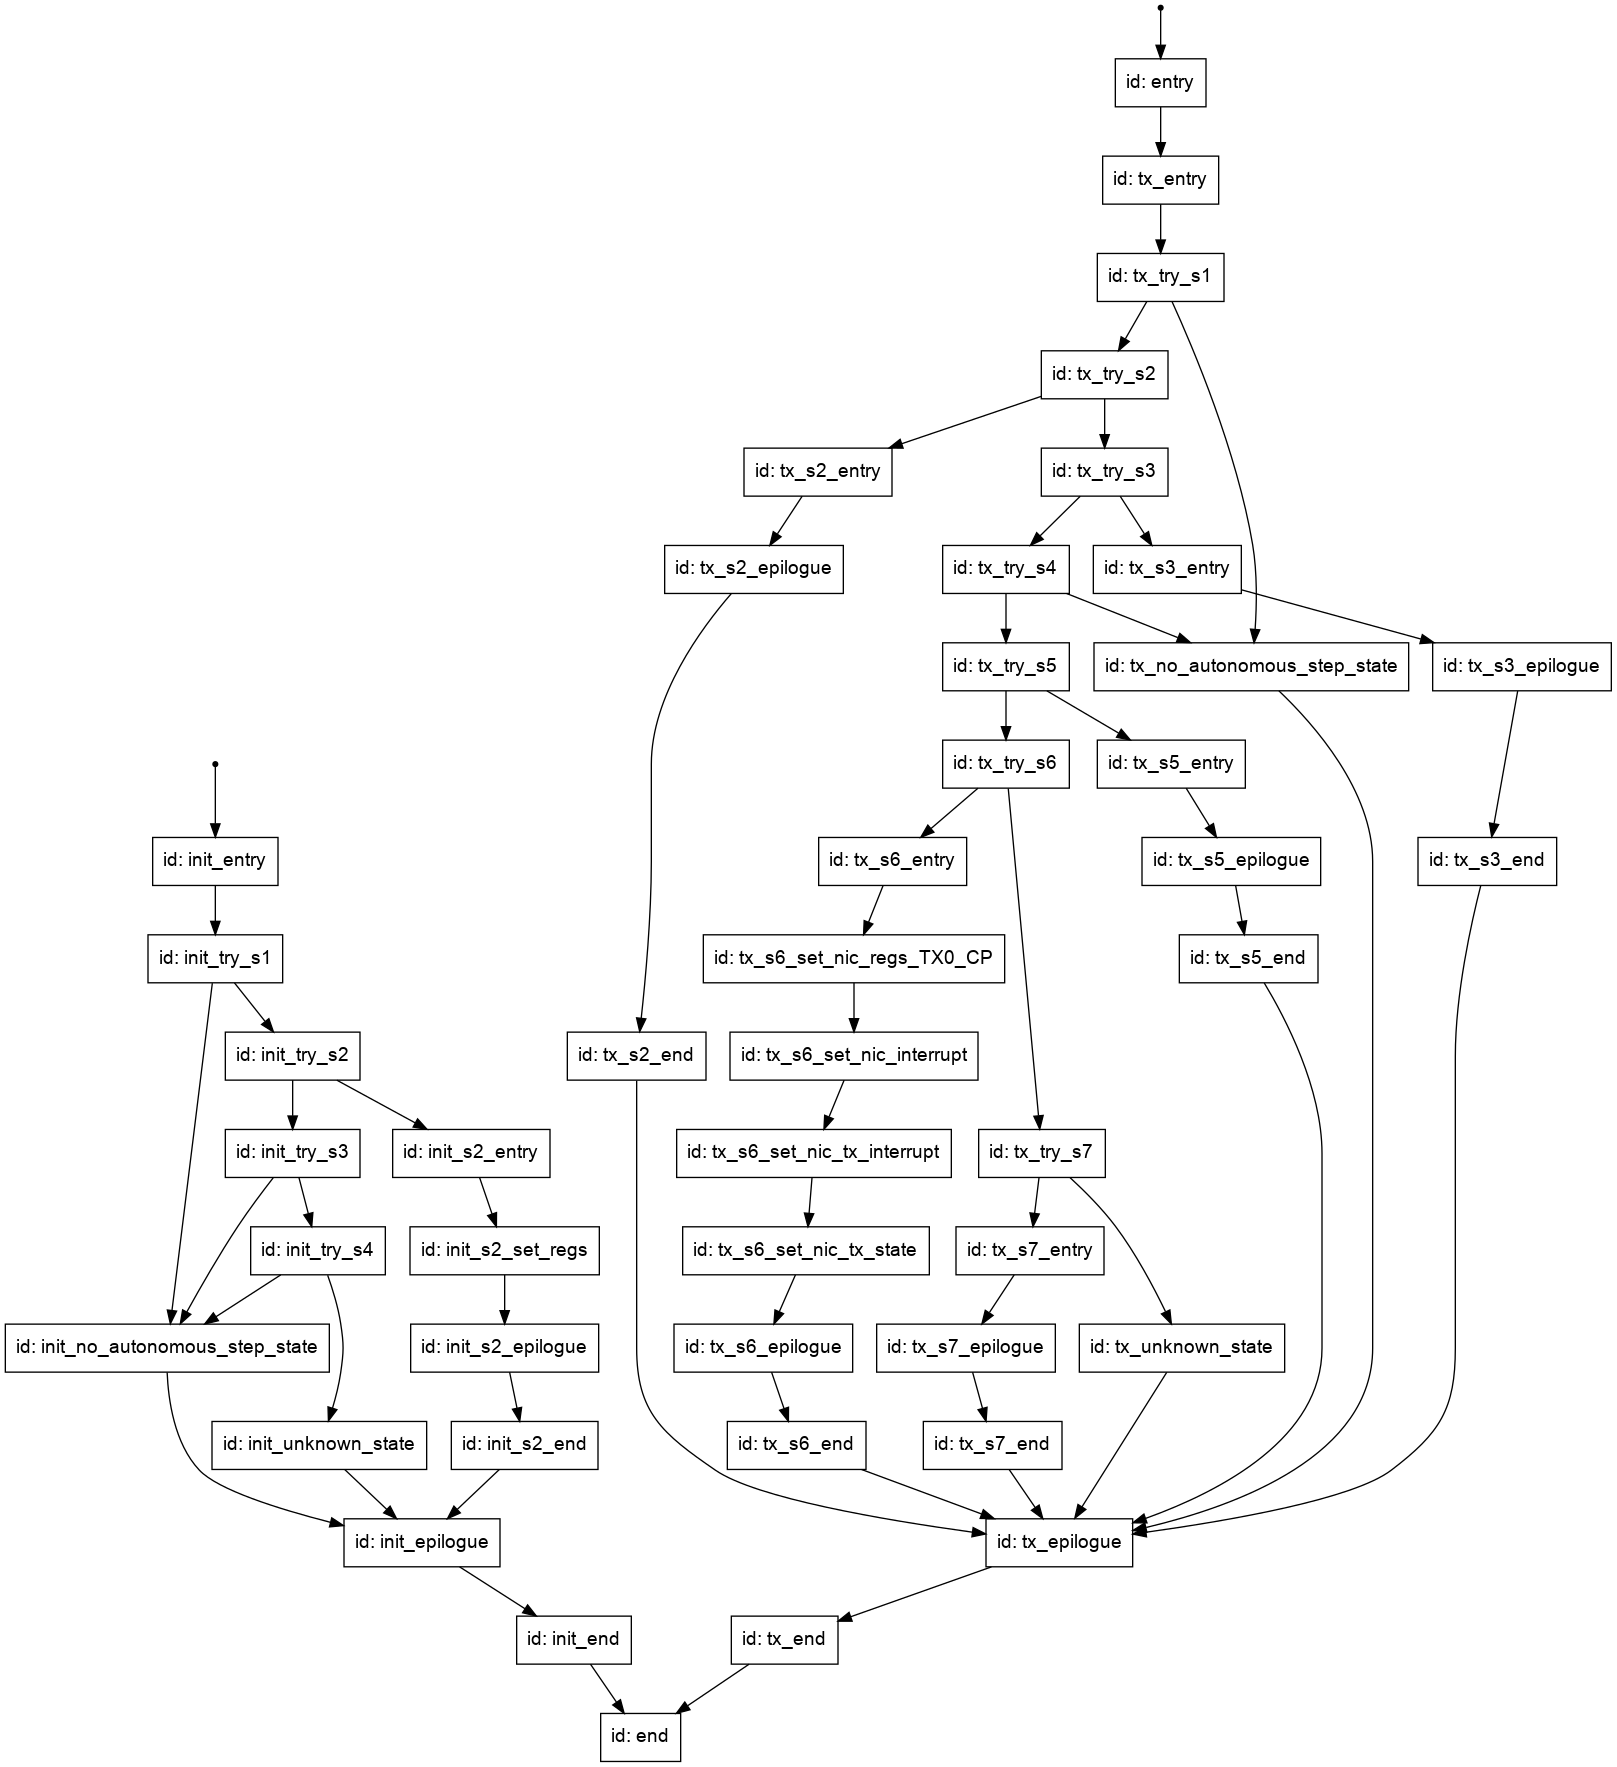
\includegraphics[width=\textwidth]{figures/nic-bir-model-cfg.png}
	\centering
	\caption{\gls{CFG} of the implemented transitions of the NIC BIR model. Each node represents one BIR block and each edge one jump target. Because the scheduler hasn't been implemented in this model, the \textbf{entry} block is jumping arbitrarily on \textit{tx\_entry}; all contract verification procedures take labels in order to define entry and end points of the section of a program that the tools should generate the weakest precondition from, so this isn't a problem in practice as long as no attempt to perform proofs on more than one automaton are made. The CFG of the full program would resemble a tree with one node at the top, \textit{entry}, and the tree getting larger with the depth because of all the conditional jumps that go to the transition being performed.}
	\label{nic-bir-model-cfg}
\end{figure}

The static and loop-free control-flow of this BIR program is very suitable for use with HolBA's weakest precondition tool in order to perform contract-based verification, as we shall see in the next chapter.


% [Proving properties]
%
% * Introduction des WP
%   - Rappels sur le WP existant dans HolBA
% * Explication de l'utilisation de SMT solver
%   - Ajout des arrays dans l'export existant
%   - Experiments with SMT (before and after array): without and with BIR
%   --- With BIR needed BIR EXP -> Words (why?)
%   ----- Non proof-producing + explain why (mention that PP has been done in the proof)
% * Non proof-producing WP lib
%   + easy
%   - proof-producing would have been feasible
%     -> but would have taken more time, that's not the aim of the thesis
% * BIR PP because huge WP BIR expressions
% * WP tests
%   - simple
%   - Gauss analysis (how to handle loop, mult problem with SMT)
%   - memories
%   - cjmp bug?
%   - explain the simp (ie. the subst theory) + the exponential growth issue ? should I explain it ?
% * Using the WP tool on simple properties on the BIR NIC model
%   - Remind about the impossibility to express certain properties using contracts
% * Explain the PP proof
%   - Whiteboard explanation
%   - Pen and paper proof
%   - About implementation
%   --- About PP BIR to words

\chapter{Contract-based verification} \label{contract-based-verif}
\vspace{-1cm}
\textit{This chapter will present contract-based verification, explaining the underlying theory: Hoare Triples, weakest precondition derivation and the use of SMT solvers. It will also present the current status of contract-based verification in HolBA, and present some of the work needed in order to reason about BIR memories with SMT solvers.}

\section{Hoare triples} \label{hoare-triples}

Contract-based verification is a powerful approach for verifying programs. For a given program $prog$ consisting of a list of instructions and two predicates $P$ and $Q$ called respectively pre- and postcondition, a Hoare triple \htriple{P}{prog}{Q} states that when executing the program $prog$ from a state $S$ terminates in a state $S'$, if $P$ holds in $S$ then $Q$ will hold in $S'$ (Equation \ref{ht_def}). Hereafter, we assume programs and states to be well-typed. A Hoare Triple is also called \textit{a contract}.

\begin{equation}
  \htriple{P}{prog}{Q} \eqdef S' = exec(S, prog) \implies P(S) \implies Q(S')
  \label{ht_def}
\end{equation}

For example, \htriple{P}{\varnothing}{P} holds because an empty program doesn't change the state of the execution. \htriple{n=1}{n:=n+1}{even(n)}, with $n \in \mathbb{N}$, holds because $1+1=2$, which is even.

In order to perform the verification, the Hoare logic introduces a set of axioms describing the effect of each instruction of a given language over the execution state \cite{hoare_axiomatic_1969}. For an assignment $x:=f$ where $x$ is a variable identifier and $f$ an expression without side-effects, Equation \ref{axiom_assignment_def} defines the axiom of assignment, where $P[f/x]$ denotes the substitution of all occurrences of $x$ by $f$ in $P$.

\begin{equation}
  \htriple{P[f/x]}{x:=f}{P}
  \label{axiom_assignment_def}
\end{equation}

%\textbf{TODO}: Introduce labels? \htriple{l1:P}{l1\rightarrow\{l2,l3\}}{l2:Q,l3:Q'}

\section{Weakest precondition derivation}

While Hoare logic introduces sufficient preconditions, Dijkstra introduced the concept of necessary and sufficient preconditions, called ``weakest'' preconditions \cite{dijkstra_guarded_1975}. Such weakest preconditions can be automatically derived from a program $prog$ and a postcondition $Q$. Let's call $\WP(prog, Q)$ such a weakest precondition. Then, from Equation \ref{ht_def} follows:

\begin{equation}
  \forall (prog, Q),
  \htriple{\WP(prog,Q)}{prog}{Q}
  \label{ht_wp_eq}
\end{equation}

For the program $n:=n+1$ mentioned in the previous section, we can generate the weakest precondition for the postcondition $even(n)$. First, we can rewrite $even(n)$ as $n~MOD~2 = 0$ with $MOD$ denoting the arithmetic modulo. Then, we derive the weakest precondition of the statement $n:=n+1$ by transforming the predicate $n~MOD~2 = 0$ by substituting all occurrences of $n$ by $n+1$:

\begin{equation}
  \WP(``n:=n+1'',n~MOD~2 = 0)=(n+1~MOD~2 = 0)
  \label{wp_comp_n_inc_even}
\end{equation}

From the properties of the modulo, we can simplify $n+1~MOD~2 = 0$ to $n~MOD~2 = 1$ or $odd(n)$. Therefore, \htriple{odd(n)}{n:=n+1}{even(n)}, i.e. incrementing the value of an odd integer variable by one makes it even.

While the triple \htriple{n=1}{n:=n+1}{even(n)} uses a sufficient precondition for establishing its postcondition, the triple \htriple{odd(n)}{n:=n+1}{even(n)} uses the weakest precondition. The later being the weakest precondition of the former, the two contracts are in relation:

\begin{equation}
  n=1 \implies odd(n)
\end{equation}

More generally, for a triple \htriple{P}{prog}{Q} to hold, $P$ must be stronger than the weakest precondition, i.e. we need to prove that $P \implies \WP(prog, Q)$:

%\textbf{TODO}: Here and above, should we mention/explain termination?

\begin{equation}
  (P \implies \WP(prog, Q)) \implies \htriple{P}{prog}{Q}
  \label{p_imp_wp}
\end{equation}

\section{Using SMT solvers to prove contracts} \label{using-smt-to-prove-contracts}

From Equation \ref{p_imp_wp} we see that, in order to prove that a triple \htriple{P}{prog}{Q}, we need to prove $P \implies \WP(prog, Q)$. While multiple methods exist to perform such proofs, \acrshort{SMT} solvers offer a convenient and automatic solution.

\gls{SMT} problem is a decision problem for logical formulas with respect to combinations of background theories such as arithmetic, bit-vectors, arrays or uninterpreted functions \cite{nikolaj_bjorner_programming_2019}. {SMT} problem is a generalization of \gls{SAT} problem supporting more theories. When given a formula, an {SMT} solver decides if the formula is satisfiable, i.e. if there exist a valuation of its variables where the formula evaluates to true. As an {SMT} solver can fail to decide a given instance, there are three possible outputs: ``satisfiable'', ``unsatisfiable'' and ``unknown''. The ability to ask for a satisfying model is another useful feature of some {SMT} solvers, which represents a counter-example of a false predicate.

A predicate $P$ holds if it evaluates to true for all possible values of its variables. Alternatively, the negation of a predicate $\neg P$ holds if there exist no valuation of its variables where the predicate evaluates to true, i.e. if the instance is unsatisfiable. Therefore, if a {SMT} solver report that $\neg P$ is ``unsatisfiable'', then $P$ holds.

Another way of thinking about how to prove logical formulas with {SMT} solvers is by using De Morgan's Laws: we know that $\neg (P \implies \WP) \equiv (P \land \neg \WP)$. Therefore, proving that $\neg (P \implies \WP)$ is ``unsatisfiable'' using an {SMT} solver can be seen as proving that there exist no model where $P$ holds and $\WP$ doesn't.

\subsection{The BitVector theory}

To reason about fixed-size integers, \gls{SMT} solvers often implement a ``BitVector'', or ``FixedSizeBitVectors'', theory. In order to understand its particularities, we can try to prove Equation \ref{bv_eq1}. Hereafter, we will use Z3, a popular and efficient {SMT} solver implemented by Microsoft Research\footnote{Z3 is available on GitHub at \url{https://github.com/Z3Prover/z3/}.}, and SMT-LIB 2.0, which is a standard format for {SMT} solvers \cite{barrett_satisfiability_2016}. Listing \ref{bv_eq1_smtlib} shows the SMT-LIB 2.0 representation of this proof attempt.

\begin{equation}
    \forall x.~ x + 1 > x, \text{with $x$ an unsigned 32-bit integer}
    \label{bv_eq1}
\end{equation}

\begin{lstlisting}[
    language=Lisp,
    backgroundcolor=\color{codebackcolour},
    commentstyle=\color{codegreen},
    keywordstyle=\color{magenta},
    stringstyle=\color{codepurple},
    label=bv_eq1_smtlib,caption=SMT-LIB 2.0 representation of Equation \ref{bv_eq1}.,
    frame=tb,basicstyle=\footnotesize\ttfamily]
(declare-const x (_ BitVec 32))
(assert (not
  (bvugt (bvadd x (_ bv1 32)) x)))
(check-sat)
(get-model)
\end{lstlisting}

When given Listing \ref{bv_eq1} as input, Z3 gives the following output:

\begin{lstlisting}[
    language=Lisp,
    backgroundcolor=\color{codebackcolour},
    commentstyle=\color{codegreen},
    keywordstyle=\color{magenta},
    stringstyle=\color{codepurple},
    label=bv_eq1_output,caption=Z3 output for Listing \ref{bv_eq1_smtlib}.,
    frame=tb,basicstyle=\footnotesize\ttfamily]
sat
(model (define-fun x () (_ BitVec 32) #xffffffff))
\end{lstlisting}

Z3 is telling us that Equation \ref{bv_eq1} is false, and gives a counterexample: $x=2^{32}-1$. Indeed, with this value of $x$, $x+1$ wraps around and result in $0$ which is smaller than $2^{32}-1$. This behavior is due to the bounded nature of fixed-size integers. The correct equation here would be:

\begin{equation}
    \forall x.~ x \neq 2^{32}-1 \implies x+1>x, \text{with $x$ an unsigned 32-bit integer}
    \label{bv_eq2}
\end{equation}

Listing \ref{bv_eq2_smtlib} and \ref{bv_eq2_output} show the input and output of Z3 used to successfully prove Equation \ref{bv_eq2}.

\begin{lstlisting}[
    language=Lisp,
    backgroundcolor=\color{codebackcolour},
    commentstyle=\color{codegreen},
    keywordstyle=\color{magenta},
    stringstyle=\color{codepurple},
    label=bv_eq2_smtlib,caption=SMT-LIB 2.0 representation of Equation \ref{bv_eq2}.,
    frame=tb,basicstyle=\footnotesize\ttfamily]
(declare-const x (_ BitVec 32))
(assert (not
  (bvugt (bvadd x (_ bv1 32)) x)))
(assert (not (= x #xffffffff)))
(check-sat)
\end{lstlisting}

\begin{lstlisting}[
    language=Lisp,
    backgroundcolor=\color{codebackcolour},
    commentstyle=\color{codegreen},
    keywordstyle=\color{magenta},
    stringstyle=\color{codepurple},
    label=bv_eq2_output,caption=Z3 output for Listing \ref{bv_eq2_smtlib}.,
    frame=tb,basicstyle=\footnotesize\ttfamily]
unsat
\end{lstlisting}

\section{Contract-based verification in HolBA} \label{contract-verif-holba}

\gls{holba} provides a \gls{proof-producing} tool for automatically deriving weakest preconditions on loop-free \gls{BIR} programs whose control flow can be statically identified \cite{lindner_trabin:_2019}. This tool is proof-producing in that it proves Theorem \ref{triple_wp_thm} which is the instantiation of Definition \ref{holba_wp_ht_thm}, with $(p,~entry\_l,~end\_ls)$ defining the program, $wp$ the derived weakest precondition, $post$ the given postcondition.

\begin{equation}
    bir\_exec\_to\_labels\_triple~prog~entry\_l~end\_ls~\mathbf{wp}~post
    \label{triple_wp_thm}
\end{equation}

\begin{small}
\begin{equation}
\begin{split}
    \vdash \forall &(prog :\alpha~bir\_program\_t)~(entry\_l :bir\_label\_t)%
    ~(end\_ls :bir\_label\_t \rightarrow bool)\\
    & (pre :bir\_exp\_t)~(post :bir\_exp\_t).\\
    & bir\_exec\_to\_labels\_triple~prog~entry\_l~end\_ls~pre~post \Leftrightarrow\\
    & ~~\forall~(s~:bir\_state\_t)~(r~:\alpha~bir\_execution\_result\_t).\\
    & ~~~~~~~~~~~~~~~~~bir\_env\_vars\_are\_initialised~s.bst\_environ~(bir\_vars\_of\_program~prog)\\
    & ~~~~~~\implies s.bst\_pc.bpc\_index~=~0~\land~s.bst\_pc.bpc\_label~=~entry\_l\\
    & ~~~~~~\implies s.bst\_status~=~BST\_Running\\
    & ~~~~~~\implies bir\_is\_bool\_exp\_env~s.bst\_environ~pre\\
    & ~~~~~~\implies bir\_eval\_exp~pre~s.bst\_environ~=~bir\_val\_true\\
    & ~~~~~~\implies bir\_exec\_to\_labels~end\_ls~prog~s~=~r\\
    & ~~~~~~\implies \exists~(obs~:\alpha~list)~(step\_count~:num)%
    ~(pc\_count~:num)~(s'~:bir\_state\_t).\\
    & ~~~~~~~~~~~~~~~~~~~~~~~~r~=~BER\_Ended~obs~step\_count~pc\_count~s'\\
    & ~~~~~~~~~~~~~~~~~~~\land~s'.bst\_status~=~BST\_Running\\
    & ~~~~~~~~~~~~~~~~~~~\land~bir\_is\_bool\_exp\_env~s'.bst\_environ~post\\
    & ~~~~~~~~~~~~~~~~~~~\land~bir\_eval\_exp~post~s'.bst\_environ~=~bir\_val\_true\\
    & ~~~~~~~~~~~~~~~~~~~\land~s'.bst\_pc.bpc\_index~=~0~\land~s'.bst\_pc.bpc\_label~\in~end\_ls
\end{split}
\label{holba_wp_ht_thm}
\end{equation}
\end{small}

It is interesting to note that this tool doesn't produce a theorem stating that the generated expression is actually \textit{the} weakest precondition. Nevertheless, in practice, this theorem isn't needed to perform contract-based verification if the generated ``weakest'' precondition is weak enough so that our precondition can imply it. However, without this theorem, it is impossible to prove that a given precondition $P$ isn't strong enough to establish the postcondition. We will still use the term ``weakest precondition'' as it is in practice how we are using this tool.

Definition \ref{holba_wp_ht_thm} introduces additional conditions about well-typedness and initialization that are needed in BIR today\footnotemark, as well as the notion of ``Block Program Counter'' for multi-statement blocks. %However, those can easily be proved and we are then left with the Hoare triple definition expressed in terms of evaluating the pre- and post-conditions in the initial and final state.

\footnotetext{Removal of the need for initialization is being discussed at the time of the writing, because actual hardware registers and memories are in facts always initialized: \url{https://github.com/kth-step/HolBA/issues/63}}

This tool doesn't provide a simple interface to compute weakest preconditions for a given program and postcondition, nor does it provide any support for proving the relation between the precondition and the weakest precondition. Then, in order to prove that the Hoare triple holds from this generated Theorem \ref{triple_wp_thm}, we need to prove:

\begin{equation}
    bir\_exec\_to\_labels\_triple~p~entry\_l~end\_ls~\mathbf{pre}~post
    \label{triple_pre_thm}
\end{equation}

Assuming well-typedness and initialization, after rewriting the definition of $bir\_exec\_to\_labels\_triple$, we have to show $bir\_eval\_exp~\mathbf{wp}~s.bst\_environ~=~bir\_val\_true$ in order to prove our goal using the \textit{modus ponens} with Theorem \ref{triple_wp_thm}. This corresponds to proving the following implication:

\begin{small}
    \begin{equation}
        \begin{split}
            &bir\_eval\_exp~\mathbf{pre}~s.bst\_environ~=~bir\_val\_true\\
            &\implies bir\_eval\_exp~\mathbf{wp}~s.bst\_environ~=~bir\_val\_true
        \end{split}
        \label{eval_pre_imp_eval_wp}
    \end{equation}
\end{small}

In Equation \ref{eval_pre_imp_eval_wp} we can recognize Equation \ref{p_imp_wp} that we discussed how to prove using \gls{SMT} solvers in Section \ref{using-smt-to-prove-contracts}. However, the expressions are expressed as BIR expressions. We then have to find a way to use an SMT solver \footnotemark. This is the focus of the following of this thesis. Section \ref{impl-non-pp-wp-lib} will use a non \gls{proof-producing} method for translating those BIR expressions into an equivalent formula that SMT solvers can work on, then focus on automating the whole verification process. Chapter \ref{trustful-nic-analysis} will complete this proof and use it to lift properties that have been proved on the BIR implementation to the \gls{NIC} model. The following Section \ref{bir-memories-with-smt-solvers} will discuss how to make proofs about BIR memories using \gls{SMT} solvers.

\footnotetext{HOL4 \textit{computeLib} provides a convenient way for turning expressions of this form into a non-BIR expressions using BIR's semantics, via its \texttt{EVAL} function. However, this approach stops working as soon as the BIR expression contains BIR memories, that are crucial for contract verification with HolBA. As such, this method will not be further mentioned in this document.}

\section{BIR memories and SMT solvers} \label{bir-memories-with-smt-solvers}

% \textbf{TODO}: Mention SMT-LIB logics?
% \textbf{TODO}: Mention proof reconstruction?

HOL4 features a library for interfacing \gls{SMT} solvers and HOL4, called \textit{HolSmtLib}. This library supports Yices 1 and Z3 as external provers. Yices 1 being an abandoned project that doesn't support SMT-LIB 2.0, we will focus on Z3 and the standard format SMT-LIB 2.0 \cite{barrett_satisfiability_2016}. While \textit{HolSmtLib} supports export for some SMT-LIB 2.0 theories, it doesn't support the \textit{ArraysEx} theory and doesn't know about BIR. In Section \ref{contract-verif-holba}, we discussed the translation from BIR expressions to \textit{wordsTheory} \footnotemark. However, this theory doesn't contain anything about memories or arrays in general. Therefore, some modifications are needed.

\footnotetext{This theory contains definitions and theorems about words, i.e. $N$-bits bounded integers.}

BIR memories are semantically defined as functions from addresses to values. HOL4's \textit{combinTheory} contains definitions and theorems about functions and function composition, that we need in order to reason about BIR memories.

There exist four types of BIR expressions operating directly on memories (cf. Listing \ref{bir_bin_exp_def} for the list of BIR expressions, and Section \ref{exporting-bir-to-smt} for a more precise discussion of the BIR semantics):

\begin{itemize}
    \item \texttt{BExp\_Den}: this operation enables reading values from the environment. It is analogous to reading registers or the memory in assembly programs. This operation is semantically equivalent to free variables that \textit{HolSmtLib} already supports.
    \item \texttt{BExp\_MemEq}: this operation is the equality binary operation on BIR memories. This operation is semantically equivalent to equality between its operands. \textit{HolSmtLib} already supports this operation.
    \item \texttt{BExp\_Store}: this operation is used to represent memory writes. It is semantically defined as successive function updates of consecutive segments of the word being stored because the length of the memory value-type can be less or equal than the length of values stored in the memory. A function update in \textit{combinTheory} is defined with Definition \ref{combin_UPDATE_def}. \textit{HolSmtLib} cannot currently export function update operations.
    \item \texttt{BExp\_Load}: this operation is used to read from memories. As a reminder, BIR memories are semantically defined as functions from addresses to values. A function application in \textit{combinTheory} is defined with Definition \ref{combin_APP_def}. Then, a memory load operation is the concatenation of multiple function application of consecutive addresses. \textit{HolSmtLib} supports function application of uninterpreted functions only.
\end{itemize}

\begin{equation}
    \vdash \forall a~b.~a~\text{=+}~b = (\lambda f~c.~\text{if}~a = c~\text{then}~b~\text{else}~f~c)
    \label{combin_UPDATE_def}
\end{equation}

\begin{equation}
    \vdash \forall x~f.~x~\text{:>}~f = f~x
    \label{combin_APP_def}
\end{equation}

We saw in the previous list that we need to implement the support for \textit{combinTheory} function update and application in the \textit{HolSmtLib} SMT-LIB 2.0 exporter. Since we only need two operations on the memory, load and store, the \textit{ArraysEx} theory is a good fit.

SMT-LIB 2.0 \cite{barrett_satisfiability_2016} defines the \textit{ArraysEx} theory using the three following axioms:

\begin{lstlisting}[
    language=Lisp,
    backgroundcolor=\color{codebackcolour},
    commentstyle=\color{codegreen},
    keywordstyle=\color{magenta},
    stringstyle=\color{codepurple},
    label=smtlib_arrayex_axioms,caption=SMT-LIB 2.0 axioms of the \textit{ArrayEx} theory.,
    frame=tb,basicstyle=\footnotesize\ttfamily]
(forall ((a (Array s1 s2)) (i s1) (e s2))
  (= (select (store a i e) i) e)) 
(forall ((a (Array s1 s2)) (i s1) (j s1) (e s2))
  (=> (distinct i j)
      (= (select (store a i e) j) (select a j))))
(forall ((a (Array s1 s2)) (b (Array s1 s2)))
  (=> (forall ((i s1)) (= (select a i) (select b i)))
      (= a b)))
\end{lstlisting}

If those axioms hold in \textit{combinTheory} then the translation is sound. \textit{combinTheory}'s \textit{UPDATE\_APPLY} theorem in Equation \ref{combin_UPDATE_APPLY} is equivalent to the first two theorems, the first and the second conjunct corresponding respectively to the first and the second axiom. The third axiom can be proved using both \textit{combinTheory}'s \textit{APP\_def} theorem (Theorem \ref{combin_APP_def}) and \textit{boolTheory}'s \textit{EQ\_EXT} theorem (Theorem \ref{bool_EQ_EXT})

\begin{equation}
    \begin{split}
        \vdash &  ~~~~ \forall a~x~f.~(a~\text{=+}~x)~f~a = x\\
               & \land \forall a~b~x~f.~a \neq b \implies ((a~\text{=+}~x)~f~b = f~b)
    \end{split}
    \label{combin_UPDATE_APPLY}
\end{equation}

\begin{equation}
    \vdash \forall f~g.~(\forall x.~f~x = g~x) \implies (f = g)
    \label{bool_EQ_EXT}
\end{equation}

Since this translation is sound, it has been added in \textit{HolSmtLib}. The translation is direct: from \texttt{:>} and \texttt{=+} to respectively \texttt{select} and \texttt{store}. Section \ref{addreq_test} presents a test using BIR memories.



\chapter{Non proof-producing automatic contract verification} \label{impl-non-pp-wp-lib}
\vspace{-1cm}
\textit{In the previous section, we learned about contract verification and the current status of \gls{holba}'s implementation. To perform verification on the \gls{NIC} model, we would like to automate the process as much as possible. \gls{holba} currently offers tools for automatic weakest precondition generation, therefore we need to close the gap between BIR expression and SMT solvers, as well as to implement a convenient interface on top.}

\section{Exporting BIR expressions to SMT solvers} \label{exporting-bir-to-smt}

As an intermediate language for formal verification, \gls{BIR} possesses a precise semantics. The semantics of BIR expressions is expressed as a set of definitions describing what are the equivalent operations using \textit{wordsTheory} and \textit{combinTheory}. For example, the semantics of binary operators in BIR is defined with the following theorems\footnotemark:

\footnotetext{Theorems \ref{bir_bin_exp_GET_OPER_def} and \ref{bir_bin_exp_def} have been reduced to only two operators and well-typed 64-bit expressions.}

\begin{small}
    \begin{equation}
        \begin{split}
            \vdash~&bir\_bin\_exp\_GET\_OPER~BIExp\_And = words\_and\\
                   &\land bir\_bin\_exp\_GET\_OPER~BIExp\_Or = words\_or\\
        \end{split}
        \label{bir_bin_exp_GET_OPER_def}
    \end{equation}
    \begin{equation}
        \begin{split}
            \vdash~&\forall (bin\_op :bir\_bin\_exp\_t)~(w1 :word64)~(w2 :word64).\\
                   &~~~~~bir\_bin\_exp~bin\_op~(Imm64~w1)~(Imm64~w2)\\
                   &~~~~~= Imm64~(bir\_bin\_exp\_GET\_OPER~bin\_op~w1~w2)
        \end{split}
        \label{bir_bin_exp_def}
    \end{equation}
\end{small}

Similarly, a set of definitions and theorems describe the semantics of operations on BIR memories. However, correct handling of endianness, alignment, and genericity over the size of memories cells and addresses, are pretty complicated to work with. The same is true for the semantics of operations on BIR variables, because of well-typedness and initialization.

For this reason---i.e. writing \gls{proof-producing} code is costly---, we decided to write a non proof-producing function \texttt{bir\_exp\_to\_words} that translates BIR expressions to the equivalent words expression. The obvious downside of such a function is that we now have to trust the translation to be sound because we no longer get any guarantee from the theorem prover. However, the development time is dramatically decreased and offers more time for experimenting. Moreover, this function can later be implemented in a proof-producing way for more trustful verification. Then, in order to have high confidence of correctness, software engineering practices apply:

\begin{itemize}
    \item write small and understandable pieces of code and compose them, and
    \item write a comprehensive suite of tests.
\end{itemize}

BIR expressions are defined as a HOL4 algebraic data type in Listing \ref{bir_exp_t_def}. Hence, in order to translate BIR expressions to words expressions, we need to handle every variant. This has been done \footnote{Code available here: \url{https://github.com/kth-step/HolBA/commit/2fcca54dcb04a20716e7697f64b5a4578f8a8af9}} using an exhaustive \texttt{if-then-else} statement\footnotemark. The code is mostly destructuring HOL4 terms and creating new \textit{wordsTheory} and \textit{combinTheory} terms. In order to obtain an easily reviewable code, a balance between expressivity and conciseness has to be carefully decided. Table \ref{bir_exp_to_words_variants_loc} shows that the length of each variant is relatively small in terms of lines of codes, from 1 line for constants to 51 for memory store expressions. This achieves the first point of the previous list.

\footnotetext{Pattern matching would have been optimal but isn't possible because of how HOL4 is embedded in SML.}

Testing of \texttt{bir\_exp\_to\_words} has been done using a set of $(bir\_exp,expected)$ couples with increasing complexity, where \texttt{bir\_exp\_to\_words} is used to translate each $bir\_exp$ and the result is compared to $expected$. Then, BIR expressions being defined as an algebraic data type, nesting of BIR expressions follows naturally. This achieves the second point of the previous list.

\begin{lstlisting}[
    label=bir_exp_t_def,caption=bir\_exp\_t definition.,
    frame=tb,basicstyle=\footnotesize\ttfamily,
    breaklines=true,postbreak=\mbox{\textcolor{red}{$\hookrightarrow$}\space}]
Datatype `bir_exp_t =
    BExp_Const      bir_imm_t
  | BExp_Den        bir_var_t

  | BExp_Cast
  	  bir_cast_t bir_exp_t bir_immtype_t

  | BExp_UnaryExp   bir_unary_exp_t bir_exp_t
  | BExp_BinExp     bir_bin_exp_t bir_exp_t bir_exp_t
  | BExp_BinPred    bir_bin_pred_t bir_exp_t bir_exp_t
  | BExp_MemEq      bir_exp_t bir_exp_t

  | BExp_IfThenElse bir_exp_t bir_exp_t bir_exp_t

  | BExp_Load       bir_exp_t bir_exp_t bir_endian_t bir_immtype_t
  | BExp_Store      bir_exp_t bir_exp_t bir_endian_t bir_exp_t`
\end{lstlisting}

\begin{table}[ht!]
    \centering
    \begin{tabular}{ | l | c | }
        \hline
        \texttt{bir\_exp\_t} variant & Lines of code\\
        \hline
        BExp\_Const & 1\\
        BExp\_Den & 21\\
        BExp\_Cast & not implemented\\
        BExp\_UnaryExp & 8\\
        BExp\_BinExp & 9\\
        BExp\_BinPred & 10\\
        BExp\_MemEq & 10\\
        BExp\_IfThenElse & 9\\
        BExp\_Load & 48\\
        BExp\_Store & 51\\
        \hline
    \end{tabular}
    \caption{Length of each \texttt{bir\_exp\_t} variant in the implementation of \texttt{bir\_exp\_to\_words}.}
    \label{bir_exp_to_words_variants_loc}
\end{table}

\section{Pretty-printing to visualize BIR expressions} \label{pretty-printers}

When working with complex constructs, the need for visualization techniques often arises. Generated weakest preconditions quickly grow with the number of statements in a program, linearly or exponentially depending on the type of statements---control flow statements produce exponential growth. While clever techniques can be implemented to keep their size reasonable \cite{lindner_trabin:_2019}, we often need to read and analyze them.

Printing of BIR terms in general is very verbose. For example, the expression \ref{pp_ex_math_exp} with a 64-bit $x$ integer defined using the BSL code in Listing \ref{pp_ex_bsl_code} yields the printing in Figure \ref{pp_ex_default_printing} using HOL4's default printing capabilities.

\begin{equation}
    \textbf{if}~~(x \leq 100) \lor (y + 1 > 10) \lor (x + y \leq 20)~~\textbf{then}~~2 \times x~~\textbf{else}~~3 \times y + 1
    \label{pp_ex_math_exp}
\end{equation}

\begin{lstlisting}[
    language=Caml,
    backgroundcolor=\color{codebackcolour},
    commentstyle=\color{codegreen},
    keywordstyle=\color{magenta},
    stringstyle=\color{codepurple},
    label=pp_ex_bsl_code,caption=BSL code,
    frame=tb,basicstyle=\footnotesize\ttfamily,
    float,floatplacement=H]
bite (
  borl [
    ble ((bden o bvarimm64) "x", bconst64 100),
    bnot (ble (bplus ((bden o bvarimm64) "y",
                      bconst64 1),
               bconst64 10)),
    ble (bplus ((bden o bvarimm64) "x",
                (bden o bvarimm64) "y"),
         bconst64 20)
  ],
  bmult ((bden o bvarimm64) "x", bconst64 2),
  bplus (bmult ((bden o bvarimm64) "x", bconst64 3),
         bconst64 1))
\end{lstlisting}

\begin{figure}[!h]
	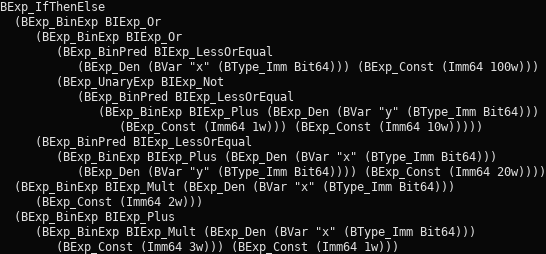
\includegraphics[width=\textwidth]{figures/pp_ex_default_printing.png}
	\centering
	\caption{Default HOL4 printing}
	\label{pp_ex_default_printing}
\end{figure}

This expression is relatively small and yet the printed term is 17 lines long. Compared to the BSL expression that is 8 lines long\footnotemark, that is a two-time increase in size. Moreover, lines are long and verbose: for example, a ``less-than'' binary expression is written as ``\texttt{BExp\_BinPred BIExp\_LessOrEqual e1 e2}''. Comparatively, the math expression ``$e1 \leq e2$'' and BSL expression ``\texttt{ble e1 e2}'' are shorter and arguably more readable.

\footnotetext{8 lines correspond to the length in documents where line length is limited to 100 characters, instead of the 60 in the report. 100 characters are the usual setting for maximum line lengths and correspond more closely to reality.}

To answer to this kind of issues, HOL4 provides the ability to implement ``pretty-printers'', which are custom printing functions for a given type. We implemented four pretty-printers in order to shorten the verbosity of the printed representation and to add colors to the output. Figure \ref{pp_ex_pretty_printing} shows the same expression printed with the pretty-printers enabled.

\begin{figure}[!h]
	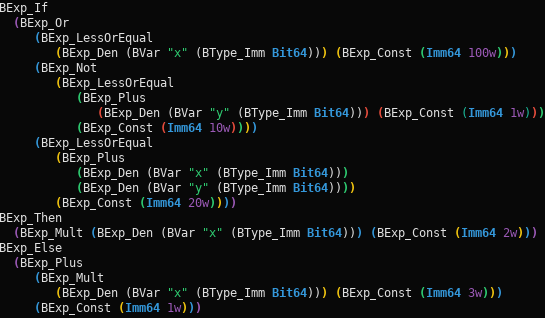
\includegraphics[width=\textwidth]{figures/pp_ex_pretty_printing.png}
	\centering
	\caption{Same expression printed with the pretty-printers enabled.}
	\label{pp_ex_pretty_printing}
\end{figure}

The pretty-printers introduce a set of features:

\begin{itemize}
    \item Simplification of verbose constructs as discussed before (e.g. \texttt{BExp\_BinExp BIExp\_Or} is written as \texttt{BExp\_Or}).
    \item Different representation of \textbf{if-then-else} statements, simplifying reading the expression when either the condition or the \textbf{then} expression are very long.
    \item Consistent breaking---new lines---of long expressions, because the default printer isn't aware of the structure of printed expressions. In Figure \ref{pp_ex_default_printing}, we can see inconsistent breaking in addition and multiplication binary operations.
    \item Highlighting of types, facilitating debugging when the expression isn't well-typed.
    \item Highlighting of all strings, facilitating reading labels and variable names.
    \item Gathering of nested binary expressions of the same type on the same level. We can see this feature in Figure \ref{pp_ex_pretty_printing} with the two nested \textbf{or} binary operators, where the three operands are printed on the same level.
    \item Rainbow parenthesis, i.e. matching pairs of parenthesis are printed in the same color. This feature is useful when reading long expressions in order to quickly identify where a sub-expression ends.
\end{itemize}

% TODO: Mention the Lisp printing attempt?

\section{Implementing a convenient interface} \label{impl_convenient_ht_interface}

In order to perform a high number of proofs on the \gls{NIC} model, we want to hide as much as possible the implementation details of the contract verification procedure. Ideally, we want a function ``\texttt{prove\_contract}'' taking a program fragment, a pre- and a post-condition as parameters, and producing a proof about the Hoare Triple if the contract holds or a comprehensive and useful error message if it doesn't. Listing \ref{ideal_interface_prove_contract} shows the ideal interface that we would want, and Listing \ref{interface_prove_contract} shows the actual interface that has been implemented.

\begin{lstlisting}[
    language=Caml,
    backgroundcolor=\color{codebackcolour},
    keywordstyle=\color{magenta},
    label=ideal_interface_prove_contract,caption=Ideal interface for ``\texttt{prove\_contract}'',
    frame=tb,basicstyle=\footnotesize\ttfamily]
fun prove_contract contract_name prog_def
    (precond_lbl, precond_bir_exp)
    postcond_lbl_and_bir_exp_list
\end{lstlisting}

\begin{lstlisting}[
    language=Caml,
    backgroundcolor=\color{codebackcolour},
    keywordstyle=\color{magenta},
    label=interface_prove_contract,caption=Actual interface for ``\texttt{prove\_contract}'',
    frame=tb,basicstyle=\footnotesize\ttfamily]
fun prove_contract contract_name prog_def
    (precond_lbl, precond_bir_exp)
    (postcond_lbl_list, postcond_bir_exp)
\end{lstlisting}

Interface in Listing \ref{ideal_interface_prove_contract} leverages the general idea of how the weakest precondition generation procedure works: it starts from end labels, setting the weakest precondition there to the postcondition, then propagate the weakest precondition of each node of the \gls{CFG} to the previous nodes, and stops when it meets the entry label. Then, it is in theory possible to provide different postconditions to each end label, hence the last parameter being a list of $(end\_label, postcond\_exp)$ pairs. However, the current tool only supports using the same postcondition for the multiple end labels, therefore the interface has been constrained\footnotemark.

\footnotetext{A proposal is being discussed at the time of writing this report about making the weakest precondition generation and the Hoare Triple definition more general, and possibly allowing this feature.}

When implementing this function, high attention has been paid to provide useful and comprehensive feedback in the case of failure. To that end, extensive use of exception wrapping has been made in order to give precise context to exceptions, and a logging library has been implemented (cf. Chapter \ref{user-friendliness}).

When used with \gls{BSL} to express pre- and post-conditions, this function provides a convenient and automatic solution to prove contracts. In the following sections, we will then see usage of this function, first to test it and then to perform proofs on the NIC model.

\section{Testing the automatic proof procedure}

We need to perform simple proofs in order to test that the proof procedure works. The following examples introduce two of the tests that have been implemented, focusing on the critical parts of each of them. To this end, some liberties have been taken in order to reduce the complexity for the reader. Moreover, even if the test on conditional jumps has been the last one introduced in chronological order \footnotemark, it will be presented first because of its relative simplicity.

\footnotetext{The test on conditional jumps has been introduced in order to fix a bug in the weakest precondition simplification library.}

\subsection{Conditional jump test} \label{cjmp_test}

Here we are interested in testing the \texttt{prove\_contract} function in the presence of a conditional jump with its condition being just an equality test. Feature-wise, this test contains only jump, conditional jump and assignment statements. Listing \ref{cjmp_test_pseudocode} gives a pseudocode representation of this test program, the conditional jump being represented with the ``\textbf{goto-if-then-else}'' construct.

\begin{lstlisting}[
    language=C,
    backgroundcolor=\color{codebackcolour},
    commentstyle=\color{codegreen},
    keywordstyle=\color{magenta},
    stringstyle=\color{codepurple},
    label=cjmp_test_pseudocode,caption=Equivalent pseudocode of the \textit{cjmp} test.,
    frame=tb,basicstyle=\footnotesize\ttfamily]
entry:
  x = 1;
  goto (if x=1 then assign_y_100 else assign_y_200)
assign_y_100:
  y = 100;
  goto end
assign_y_200:
  y = 200;
  goto end
end:
\end{lstlisting}

In this test, we want to check that the triple \htriple{\top}{prog}{y = 100} holds. Intuitively, this contract means ``for every possible initial state $S$, executing the program will result in a state $S'$ with $y=100$''. It is interesting to note that the precondition $\top$ means ``for every initial state'', analogous to the universal quantifier $\forall$ in logic. This comes from the fact that $\top$ is the weakest precondition possible: $\forall x.~x \implies \top$. Thus, for this Hoare Triple to hold, the generated weakest precondition must be $\top$. Listing \ref{cjmp_test_prove_contract_call} shows the invocation of \texttt{prove\_contract}.

\begin{lstlisting}[
    language=Caml,
    backgroundcolor=\color{codebackcolour},
    commentstyle=\color{codegreen},
    keywordstyle=\color{magenta},
    stringstyle=\color{codepurple},
    label=cjmp_test_prove_contract_call,
    caption=Invocation of \texttt{prove\_contract} for the \textit{cjmp} test.,
    frame=tb,basicstyle=\footnotesize\ttfamily,
    float,floatplacement=H]
val thm = prove_contract "cjmp"
  cjmp_prog_def
  (* Precondition *) (blabel_str "entry", btrue)
  (* Postcondition *) (
    [blabel_str "end"],
    beq ((bden o bvarimm32) "y", bconst32 100)
  )
\end{lstlisting}

Figure \ref{test_cjmp_bir} shows the auto-generated BIR $P \implies \WP$ expression, and Equation \ref{test_cjmp_words} shows the same expression after translation to a \textit{wordsTheory} expression. This expression can be trivially simplified to $\top$, what SMT solvers can very efficiently do. Hence, this invocation to \texttt{prove\_contract} succeeds.

\begin{figure}[!h]
	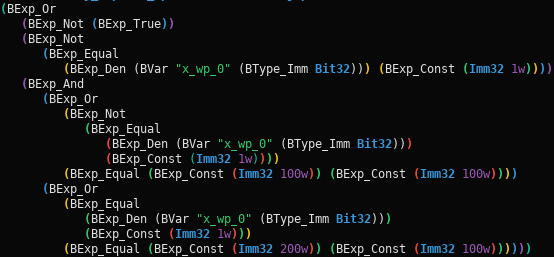
\includegraphics[width=\textwidth]{figures/test_cjmp_bir.png}
	\centering
	\caption{Auto-generated $P \implies \WP$ BIR expression for the \textit{cjmp} test.}
	\label{test_cjmp_bir}
\end{figure}

\begin{equation}
    \top \lor
    (\neg(x = 1w) \lor ((\neg(x = 1w) \lor 100w = 100w) \land (x = 1w \lor 200w = 100w)))
    \label{test_cjmp_words}
\end{equation}

\subsection{Load and store test} \label{addreq_test}

The \gls{NIC} manipulating a buffer descriptor queue, represented in BIR using memories, we need to ensure that \texttt{prove\_contract} works with programs containing memories. In this test, we will store a number $N$ in memory at address $A$, then load a number into $x$ from address $B$. We want to check the following Hoare Triple: \htriple{A=B}{prog}{x=N}. Listing \ref{test_addreq_pseudocode} shows the equivalent pseudocode of the test program, Figure \ref{test_addreq_bir} the auto-generated $P \implies \WP$ expression, Figure \ref{test_addreq_words} the same expression translated in \textit{wordsTheory} and Listing \ref{test_addreq_smtlib} the auto-generated SMT-LIB 2.0 instance featuring \texttt{select} and \texttt{store} operations.

\begin{lstlisting}[
    language=C,
    backgroundcolor=\color{codebackcolour},
    commentstyle=\color{codegreen},
    keywordstyle=\color{magenta},
    stringstyle=\color{codepurple},
    label=test_addreq_pseudocode,caption=Equivalent pseudocode of the \textit{load and store} test,
    frame=tb,basicstyle=\footnotesize\ttfamily]
MEM = store(MEM, ADDR1, 42)
x = load(MEM, ADDR2)
\end{lstlisting}

\begin{figure}[!h]
	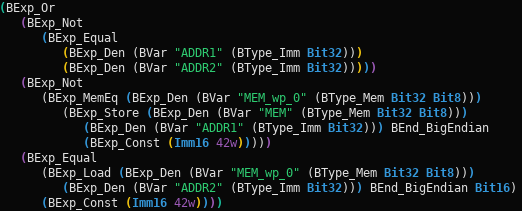
\includegraphics[width=\textwidth]{figures/test_addreq_bir.png}
	\centering
	\caption{Auto-generated $P \implies \WP$ BIR expression for the \textit{load and store} test.}
	\label{test_addreq_bir}
\end{figure}

\begin{figure}[!h]
	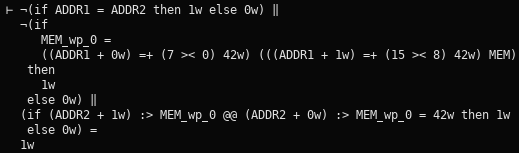
\includegraphics[width=\textwidth]{figures/test_addreq_words.png}
	\centering
	\caption{$P \implies \WP$ expression translated in \textit{wordsTheory} for the \textit{load and store} test. \texttt{><} is the bitwise extraction operation, \texttt{@@} the word concatenation operation, \texttt{=+} the memory update operation and \texttt{:>} the memory load operation (cf. Section \ref{bir-memories-with-smt-solvers}). Bit extraction and concatenation is needed because we are working with 16-bit words in a 8-bit memory.}
	\label{test_addreq_words}
\end{figure}

\begin{lstlisting}[
    language={},
    backgroundcolor=\color{codebackcolour},
    commentstyle=\color{codegreen},
    keywordstyle=\color{magenta},
    stringstyle=\color{codepurple},
    label=test_addreq_smtlib,caption=Autogenerated SMT instance for the \textit{load and store} test,
    frame=tb,basicstyle=\footnotesize\ttfamily,
    float,floatplacement=H,
    breaklines=true,postbreak=\mbox{\textcolor{red}{$\hookrightarrow$}\space}]
(set-info :source |Automatically generated from HOL4 by SmtLib.goal_to_SmtLib.
Copyright (c) 2011 Tjark Weber. All rights reserved.|)
(set-info :smt-lib-version 2.0)
(declare-fun v0_ADDR1 () (_ BitVec 32))
(declare-fun v1_ADDR2 () (_ BitVec 32))
(declare-fun v2_MEM_wp_0 ()
  (Array (_ BitVec 32) (_ BitVec 8)))
(declare-fun v3_MEM ()
  (Array (_ BitVec 32) (_ BitVec 8)))
(assert
 (not
  (=
   (bvor
    (bvnot (ite (= v0_ADDR1 v1_ADDR2)
                (_ bv1 1) (_ bv0 1)))
    (bvor
     (bvnot
      (ite
       (= v2_MEM_wp_0
        (store
         (store
          v3_MEM
          (bvadd v0_ADDR1 (_ bv1 32))
          ((_ zero_extend 0) ((_ extract 15 8) (_ bv42 16))))
         (bvadd v0_ADDR1 (_ bv0 32))
         ((_ zero_extend 0) ((_ extract 7 0) (_ bv42 16)))))
       (_ bv1 1)
       (_ bv0 1)))
     (ite
      (=
       (concat
        (select v2_MEM_wp_0 (bvadd v1_ADDR2 (_ bv1 32)))
        (select v2_MEM_wp_0 (bvadd v1_ADDR2 (_ bv0 32))))
       (_ bv42 16))
      (_ bv1 1)
      (_ bv0 1))))
   (_ bv1 1))))
(check-sat)
(exit)
\end{lstlisting}

This expression is harder to prove manually. However, SMT solvers can report very efficiently that the negated expression is unsatisfiable, proving the contract. Therefore, we see that contracts involving BIR memories can be proved, thanks to the work of Section \ref{bir-memories-with-smt-solvers}.

Other preconditions have been tested to verify that \texttt{prove\_contract} doesn't prove false contracts and succeeds to prove true ones. With the current program, the precondition $load(MEM,B=N)~\land~B=A+2$ can establish the postcondition. The second conjunct is important because $N$ is stored in two consecutive 8-bit memory locations. Interestingly, the precondition $\bot$ works for all contracts, because $\forall x.~\bot \implies x$, and it works in this particular case.

% TODO? \subsubsection{Gauss}
% If yes, change "two" to "three" in the subsection intro

\section{Simple automatized proofs on the NIC model} \label{simple-automated-proofs-on-nic}

Chapter \ref{nic-model} presented the implementation of parts of the NIC model using BIR. The previous sections of this chapter presented the non \gls{proof-producing} contract verification library that has been implemented. This section will present some of the properties that have been proved on the NIC BIR model. However, as we shall see, \texttt{prove\_contract} has some intrinsic limitations that prevent verifying some contracts.

Section \ref{overview-nic-proof} presents an overview of the formal HOL4 proof made in \cite{haglund_formal_2016} on the formal NIC model. We saw that the properties are phrased in terms of invariants holding in each transition of the model. Such properties can be represented as Hoare Triples and therefore can be proved using this chapter's non proof-producing contract verification library as long as the pre- and post-conditions can be represented using BIR.

In this section, we will see that the non proof-producing function \texttt{prove\_contract} is able to verify some invariants on the NIC BIR model. We will perform the verification of the Hoare Triples shown in Equations \ref{nonpp-goal-1} and \ref{nonpp-goal-2}. Those two Hoare Triple respectively represent that, stating from a non-dead initial NIC state, performing one autonomous transition of the transmission automaton doesn't end in an undefined state (i.e. a dead state) and performing one non-autonomous transition of the initialization automaton does end in an undefined state.

\begin{multline}
	\{\neg NIC.dead \land NIC.tx.state \in \{tx2,~tx3,~tx5,~tx6,~tx7\}\}\\
	tx\_automaton\{\neg NIC.dead\}
    \label{nonpp-goal-1}
\end{multline}

\begin{multline}
	\{\neg NIC.dead \land NIC.init.state \in \{it1,~it3,~it4\}\}\\
	init\_automaton\{NIC.dead\}
    \label{nonpp-goal-2}
\end{multline}

Listing \ref{nonpp-code-1} shows the SML code used to prove the first contract. Code for the other contract is similar. This example shows that the library implemented in the chapter fulfills its goal of being simple to use and fully automatic when given a Hoare Triple and a program. Combined with BSL and custom helper functions, it becomes easy to express the pre- and post-conditions, and it is still possible to use arbitrary SML functions or HOL4 terms.

\begin{lstlisting}[
    language=Caml,
    backgroundcolor=\color{codebackcolour},
    commentstyle=\color{codegreen},
    keywordstyle=\color{magenta},
    stringstyle=\color{codepurple},
    label=nonpp-code-1,caption={SML code used to prove contract \ref{nonpp-goal-1}.},
    frame=tb,basicstyle=\footnotesize\ttfamily]
(* TX automaton: NIC doesn't die in autonomous transition *)
val (_, _, p_imp_wp_word_thm) = prove_contract
  "tx_automaton_doesnt_die"
  nic_program_def
  (* Precondition *) (
    blabel_str "tx_entry",
    bandl [
      invariant_nic_not_dead,
      borl (List.map
        (fn s => beq (bdenstate "nic_tx_state",
                      bstateval_tx s))
        (#autonomous_step_list tx_state))
    ])
  (* Postcondition *) (
    [blabel_str "tx_end"],
    invariant_nic_not_dead
  )
val _ = info "Successfully proved: tx automaton doesn't die"
val _ = if !level_log >= logLib.INFO
  then (pprint_thm p_imp_wp_word_thm)
  else ();
\end{lstlisting}

\subsection{Limitations of this approach}

While being convenient and working well for simple contracts, the contract verification library implemented in this chapter suffers from two limitations:

\begin{itemize}
	\item The first one is straightforward: this library isn't \gls{proof-producing}. Using HOL4 requires a significant learning effort, and easier non proof-producing tools exist. Hence, when using HOL4, one usually wants to reason about proofs, and this library is not proof-producing and could, therefore, introduce subtle bugs or inconsistencies. Moreover, this library doesn't offer the possibility to compose Hoare Triples because it doesn't output any related theorem. If one wanted to do so, an oracle would have to be used in order to generate such theorems and enabling theorem composition and further reasoning. Nevertheless, as already explained, proof-producing code is more costly. The desired level of trustworthiness should be carefully decided, and this library offers a pragmatic solution.
	\item Secondly, this library, with its approach to contract-based verification, is limited by the expressiveness of BIR, since the pre- and post-conditions are BIR terms. BIR doesn't have quantifiers, and it is, therefore, impossible to prove contracts containing existential quantifiers. The existing formal proof on the NIC of \cite{haglund_formal_2016} requires existential quantifiers in order to reason about the buffer descriptor queue in the \textit{CPPI\_RAM} memory of the NIC, and this part of the proof can therefore not be replaced by using \texttt{prove\_contract}. Moreover, as explained in the first point of this list, composing verification produced with this library with raw HOL4 proofs is not straightforward. The following Chapter \ref{trustful-nic-analysis} explores a new proof-producing approach for performing contract-based verification of the BIR model that answers this issue.
\end{itemize}

\chapter{Trustful analysis on the NIC model} \label{trustful-nic-analysis}
\vspace{-1cm}
\textit{In the previous chapter, we implemented an automated non \gls{proof-producing} contract verification library, the non proof-producing part being the translation from BIR expressions to the equivalent \textit{wordsTheory} and \textit{combinTheory} expression. Moreover, this verification library can only produce contracts on BIR programs. In order to perform trustworthy verification on the \gls{NIC} model, we need to make proofs directly on the \gls{NIC} state. In this chapter, we will perform a proof on a BIR program and then lift it to the \gls{NIC} model.}

%bisimulation and lifting are recurring ideas in trustful binary verification.

In order to prove the feasibility of this approach, we will prove a simple property. Listing \ref{proof_nic_state} contains the NIC state on which we want to prove a property, Equations \ref{proof_nic_P_def}, \ref{proof_nic_Q_def} and \ref{proof_goal} present the property that we want to prove, and Listing \ref{proof_prog} contains a pseudocode representation of the BIR program on which we will perform the verification. Figure \ref{proof_schema} gives a visualization of the structure of the verification and the steps that we will take during the proof. 

\begin{lstlisting}[
    language={},
    backgroundcolor=\color{codebackcolour},
    commentstyle=\color{codegreen},
    keywordstyle=\color{magenta},
    stringstyle=\color{codepurple},
    label=proof_nic_state,caption=NIC state used in this proof,
    frame=tb,basicstyle=\footnotesize\ttfamily]
Datatype `nic_state = <|
  dead : bool;
  x : word32
|>`
\end{lstlisting}

\begin{small}
\begin{align}
\label{proof_nic_P_def}
\vdash~&\forall nic.~P_{NIC}~nic \eqdef \neg nic.dead \land nic.x = 0w\\
%
\label{proof_nic_Q_def}
\vdash~&\forall nic~nic'.~Q_{NIC}~nic~nic' \eqdef \neg nic'.dead \land nic'.x = nic.x + 1w\\
%
\label{proof_goal}
\vdash~&\forall nic~nic'.~P_{NIC}~nic~\land~exec\_prog~nic~bir\_prog~nic'~\implies~Q_{NIC}~nic~nic'
\end{align}
\end{small}

\pagebreak

\begin{lstlisting}[
    language=C,
    backgroundcolor=\color{codebackcolour},
    commentstyle=\color{codegreen},
    keywordstyle=\color{magenta},
    stringstyle=\color{codepurple},
    label=proof_prog,caption=Pseudocode of the program used in this proof,
    frame=tb,basicstyle=\footnotesize\ttfamily]
nic.x := nic.x + 1
if nic.x > 10:
    nic.dead := true
\end{lstlisting}

\begin{figure}[!h]
	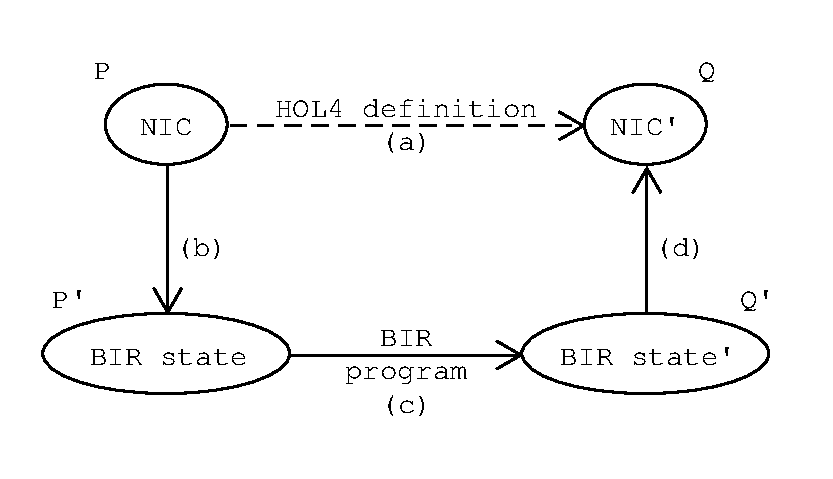
\includegraphics[height=5cm]{figures/proof_schema.pdf}
	\centering
	\caption{Visual structure of the proof. References like (a) to the arrows of this Figure are used throughout the proof to refer to a particular step.}
	\label{proof_schema}
\end{figure}

\begin{remark} \label{remark_Q_nic_intial_final}
$Q_{NIC}~nic~nic'$ is defined on both initial and final states, in order to be able to reason about the initial state in the postcondition. This allows us to write $nic'.x = nic.x + 1w$ instead of $nic'.x = 1w$ for example.
\end{remark}

Equation \ref{proof_goal} uses a relation $exec\_prog$ that we shall define now. As we want to make a proof on an undefined HOL4 definition (a), we must establish an equivalence between the HOL4 definition (a) and the BIR program (c). In real proofs, this can either be produced by a lifter which generates the BIR program from a given input program and gives a ``certificate'', i.e. a theorem stating the equivalence, or be a definition which would then mean that we trust that the BIR program is equivalent to the HOL4 definition. In this proof, we will use a definition. This definition shall state that $exec\_prog~nic~bir\_prog~nic'$ (a) is equivalent to executing the BIR program from a state $bir\_state$ to a state $bir\_state'$ (c), where $nic$ is somehow equivalent to $bir\_state$ (b) and $nic'$ somehow equivalent to $bir\_state'$ (d). To express an equivalence between HOL4 states (``$nic$'') and BIR states, we introduce a relation $R$. The relation $R~nic~bir\_state$ is defined as a simple mapping between the BIR state and the NIC state, as shown in Listing \ref{proof_R_def}. Then, we define the relation $exec\_prog$ as shown in Equation \ref{proof_eq_thm}\footnotemark.

\footnotetext{Definition \ref{proof_eq_thm} has been annotated to visualize how it is connected to the structure of the proof on Figure \ref{proof_schema}. In addition, the $BIR\_exec$ relation is used as a shorthand for $bir\_exec\_to\_labels$ in order to simplify the proof.}

\pagebreak

\begin{lstlisting}[
    language=C,
    backgroundcolor=\color{codebackcolour},
    commentstyle=\color{codegreen},
    keywordstyle=\color{magenta},
    stringstyle=\color{codepurple},
    label=proof_R_def,caption=Definition of the relation $R$,
    frame=tb,basicstyle=\footnotesize\ttfamily]
val R_def = Define `
  R (nic: nic_state) (bir_state: bir_state_t) <=>
       (bir_env_lookup "nic_dead" bir_state.bst_environ
          = SOME (BType_Bool,
                  SOME (BVal_Imm (Imm1 nic.dead))))
    /\ (bir_env_lookup "nic_x" bir_state.bst_environ
          = SOME (BType_Imm Bit32,
                  SOME (BVal_Imm (Imm32 nic.x))))`
\end{lstlisting}

\begin{small}
\begin{equation}
\begin{split}
  \vdash \forall nic~nic'. &~exec\_prog~nic~bir\_prog~nic' ~~~~~~~~~~~~~~~~~~~~~~~~~~~~~~~~~~ \text{(a)}\\
    \eqdef~&\forall bir\_state~bir\_state'.\\
          & ~~~~~~ (R~nic~bir\_state ~~~~~~~~~~~~~~~~~~~~~~~~~~~~~~~~~~~~~~~~~~~~~~~~~ \text{(b)}\\
          & ~~~~~~ \land bir\_state' = BIR\_exec~prog~bir\_state) ~~~~~ \text{(c)}\\
          & ~~~~~~ \implies R~nic'~bir\_state' ~~~~~~~~~~~~~~~~~~~~~~~~~~~~~~~~~~~~~~ \text{(d)}
\end{split}
\label{proof_eq_thm}
\end{equation}
\end{small}

\begin{proof}[Proof of Equation \ref{proof_goal}]

\numberwithin{equation}{theorem} % Changes numbering of equations inside theorems

%\textit{\textbf{Note}: The proof has been simplified in order to focus on its global structure.}

In order to begin the proof, as the goal \ref{proof_goal} is defined over $nic$ states, we need a theorem about the injectivity of the relation $R$, stating that for all $nic$ exists a $bir\_state$ such as $R~nic~bir\_state$ (b). Additionally, the $BIR\_exec$ relation will also need some properties on $bir\_state$, that we shall add in this injectivity theorem now.

\begin{theorem} \label{proof_R_inj_thm}
Injectivity theorem of $R$
\begin{equation*} \label{proof_R_inj_thm_eq}
\begin{split}
    \vdash~\forall nic.&~\exists bir\_state.\\
    		&~~~~~R~nic~bir\_state\\
		&\land~bir\_state.bst\_pc.bpc\_index = 0\\
		&\land~bir\_state.bst\_pc.bpc\_label = entry\_label\\
		&\land~bir\_state.bst\_status = BST\_Running
\end{split}
\end{equation*}
\end{theorem}

\begin{proof}
After rewriting the relation $R$, we prove theorem \ref{proof_R_inj_thm} by exhibiting a satisfying $bir\_state$.
\end{proof}

In possession of a $bir\_state$ in relation with a $nic$, we now need to lift the precondition $P_{NIC} nic$ on this $bir\_state$. First, we need to introduce equivalent pre- ---and post- ---conditions on the BIR states, then we shall prove that the precondition lifts.

\pagebreak

\begin{lstlisting}[
    language=C,
    backgroundcolor=\color{codebackcolour},
    commentstyle=\color{codegreen},
    keywordstyle=\color{magenta},
    stringstyle=\color{codepurple},
    label=proof_bir_conditions,caption=Equivalent pre- and postconditions on BIR states,
    frame=tb,basicstyle=\footnotesize\ttfamily]
val BIR_P_exp_def = Define `BIR_P_exp = ^(bandl [
  beq ((bden o bvarimm1) "nic_dead", bfalse),
  beq ((bden o bvarimm32) "nic_x", bconst32 0)
])`
val BIR_Q_exp_def = Define `BIR_Q_exp = ^(bandl [
  beq ((bden o bvarimm1) "nic_dead", bfalse),
  beq ((bden o bvarimm32) "nic_x", bconst32 1)
])`
val BIR_P_def = Define `BIR_P bstate =
  bir_eval_bool_exp BIR_P_exp bstate.bst_environ`
val BIR_Q_def = Define `BIR_Q bstate =
  bir_eval_bool_exp BIR_Q_exp bstate.bst_environ`
\end{lstlisting}

\paragraph{Limitation} $Q_{BIR}$ is a function of the end state only. Hence, in order to reason about the initial state, we need in general to introduce ghost variables in the postcondition. In this proof, since the contract that we are proving is simple, using the actual value of $nic.x$ is enough. However, this may pose a problem if we want to generalize the proof.

\paragraph{Notation} $P_{BIR}~bir\_state$ and $Q_{BIR}~bir\_state$ are defined using $bir\_eval\_bool\_exp$, which evaluates respectively the expressions $P^{exp}_{BIR}$ and $Q^{exp}_{BIR}$ in a given BIR state. In order to simplify the proof, let's define a new operator $\eqeval$ that is used to evaluate given variables, e.g. $bir\_state.x \eqeval 0w$.
\bigskip

\begin{theorem} \label{proof_b_thm}
Lifting of $P_{NIC}~nic$ to $bir\_state$
\begin{equation*} \label{proof_b_thm_eq}
\begin{split}
\vdash~\forall bir\_state~(\exists nic.~R~nic~bir\_state~\land~P_{NIC}~nic) \implies P_{BIR}~bir\_state
%⊢ ∀bir_state. (∃nic. R nic bir_state ∧ NIC_P nic) ⇒ BIR_P bir_state
\end{split}
\end{equation*}
\end{theorem}

\begin{proof}
Let's do this proof in a backward way. By using the existential elimination inference rule and discharging the antecedent of the implication, we get as assumptions $P_{NIC}~nic$ and $R~nic~bir\_state$. From this, we can deduce that $bir\_state.x \eqeval 1w$ and $bir\_state.dead \eqeval \bot$. Then, we can substitute those values in the goal, which then evaluates to $\top$.
\end{proof}

Assuming that we have a Hoare Triple theorem between initial and final BIR states, we can use Definition \ref{proof_eq_thm} in order to establish that $R~nic'~bir\_state'$. Then, in order to prove $Q_{NIC}~nic$ (d), we have to transfer the postcondition back from $bir\_state$ to $nic$.

\begin{theorem} \label{proof_d_thm}
Lowering $Q_{BIR}~bir\_state$ to $nic$.
\begin{equation*} \label{proof_d_thm_eq}
\begin{split}
\vdash~\forall~&bir\_state'.~Q_{BIR}~bir\_state' \implies\\
	&(\forall nic~nic'~bir\_state.~P_{BIR}~bir\_state\\
	&~~~~~~\land~R~nic~bir\_state~\land~R~nic'~bir\_state'\\
	&~~~\implies Q_{NIC}~nic~nic')
\end{split}
\end{equation*}
We introduce $bir\_state$ and $P_{BIR}$ in this theorem for the reason explained in Remark \ref{remark_Q_nic_intial_final}, i.e. reason about both the initial and final state in the postcondition.
\end{theorem}

\begin{proof}
This proof has been done in HOL4. The reasoning is quite similar to the proof of Theorem \ref{proof_b_thm}, as the backward proof mainly involves rewriting and simplification. We will omit this proof here and redirect the reader to the HOL4 proof available in our source repository \cite{lacroix_trustful_2019}.
\end{proof}

We will now prove that the Hoare Triple holds on the BIR program.
\bigskip

\begin{theorem} \label{proof_ht_thm}
\htriple{P^{exp}_{BIR}}{bir\_prog}{Q^{exp}_{BIR}}
\end{theorem}

\begin{proof}
To prove this Hoare Triple, we used the \gls{proof-producing} procedure implemented in \gls{holba} in order to generate the weakest precondition. The automatically derived weakest precondition is shown in Figure \ref{proof_wp_exp}. Section \ref{contract-verif-holba} already discussed how to perform this proof: we have to prove Equation \ref{eval_pre_imp_eval_wp} with $\mathbf{wp}$ being the expression in Figure \ref{proof_wp_exp} and $\mathbf{pre}$ being $P^{exp}_{BIR}$. Because we want to use an \gls{SMT} solver, we need to turn the goal of the backward proof into a \textit{wordsTheory} expression. \textit{combinTheory} isn't needed in this case since BIR memories are not used. Equation \ref{eval_pre_imp_eval_wp} uses $bir\_eval\_exp$ which evaluates an expression in the given BIR state. Therefore, to translate the goal into a \textit{wordsTheory} expression, we need to use BIR's semantics. The semantics needs well-typedness and initialization of the variables. At the time of writing, HolBA offers no support for automatic rewriting with the semantics definitions, so multiple lemmas about initialization, well-typedness, and type equality must be manually proved for every variable. Those are not shown here because they consist of simple rewriting and simplification.

\begin{figure}[!h]
	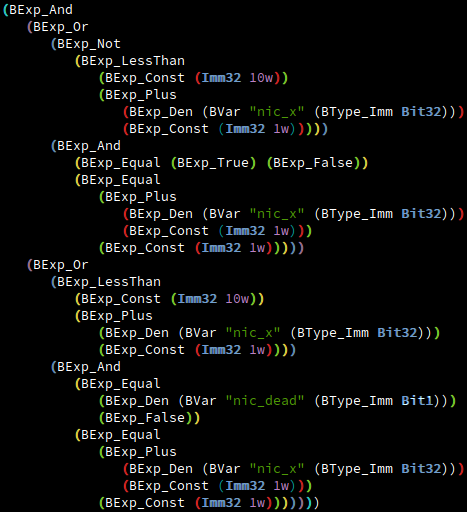
\includegraphics[scale=.65]{figures/proof_wp_exp.png}
	\centering
	\caption{Autogenerated weakest precondition for proof of Theorem \ref{proof_ht_thm}.}
	\label{proof_wp_exp}
\end{figure}

Then, the proof consist of consecutively rewriting following the definition of $bir\_eval\_exp$ and the definition it uses until the goal only contains $$bir\_env\_read~(BVar~``nic\_x"~(BType\_Imm~Bit32))~bir\_state.bst\_environ$$ and similarly for $nic.dead$. Let's call those expressions $x\_val$ and $dead\_val$ respectively. For expressions, BIR semantics is defined over immutable and constant values. Therefore, we need to establish an equivalence between the values that we currently have.

\begin{lemma}
	\begin{equation*}
		\exists x\_imm.~x\_val = BVal\_Imm~x\_imm
	\end{equation*}
	\label{proof_exists_x_imm}
\end{lemma}
\begin{proof}
Assuming well-typedness and initialization, this theorem immediately results from the BIR semantics.
\end{proof}

\begin{lemma}
	\begin{equation*}
		\exists x\_word.~x\_imm = Imm32~x\_word
	\end{equation*}
	\label{proof_exists_x_word}
\end{lemma}
\begin{proof}
This lemma is part of the BIR semantics, as one of the six conjuncts of the \texttt{bir\_imm\_t\_nchotomy} theorem, which establishes this existence theorem for every BIR immutable types.
\end{proof}

Now, using Lemmas \ref{proof_exists_x_imm} and \ref{proof_exists_x_word}, we are able to substitute all occurrences of $x\_val$ into $BVal\_Imm~(Imm32~x\_word)$, and similarly for $dead\_val$. Finally, rewriting the goal using the full set of BIR semantics theorems and some rewriting rules, the goal reduces to an expression free of BIR terms:

\begin{equation} \label{proof_wp_word_goal}
\begin{split}
&(dead\_w = 0w) \land (x\_w = 0w) \implies\\
&\Big(\neg(10w <_{+} x\_w + 1w) \lor \big((1w = 0w) \land (x\_w + 1w = 1w)\big)\Big)~\land\\
&\Big((10w <_{+} x\_w + 1w) \lor \big((dead\_w = 0w) \land (x\_w + 1w = 1w)\big)\Big)
\end{split}
\end{equation}

An \gls{SMT} solver is able to prove this goal. Interestingly, HOL4 simplification procedures are also able to prove it. However, they won't be able to prove it for more complicated ones or will be less effective than SMT solvers.
\end{proof} % End of Hoare Triple proof

Finally, using the deduction rule with Theorems \ref{proof_R_inj_thm}, \ref{proof_b_thm}, \ref{proof_R_def}, \ref{proof_ht_thm}, \ref{proof_eq_thm} and \ref{proof_d_thm}, in that order, concludes this proof.
\renewcommand\qedsymbol{$\blacksquare$}
\end{proof}

\chapter{User experience and good practices} \label{user-friendliness}
\vspace{-1cm}
\textit{This chapter will present the care that has been put into user experience and good practices throughout this work.}

% User experience
% * BSL
% * pretty printer
% * logging utilities
% * error handling (guidelines SML + HOL4)
% * exception printer
%
% Best practices: critical to build lasting complex systems
% * simple interfaces: CFG lig and WP tool
% * Git workflow
% * CI: regression tests + static analysis (insight into the code)

% The need arose in general when debugging HOL4 code for tracing code.
% LogLib is a higher-level implementation of HOL4 tracing system. Verbosity levels are specified and output is colored, helping to read long outputs.

In this work, we took the role of a user of the HolBA platform, and of HOL4 by necessity. HOL4 learning curve is quite steep, and very few efforts have been invested towards beginner friendliness because this topic can become really time-consuming and its perceived importance greatly depends on one's experience. Throughout our design and implementation process, great care has been put into having a good user experience while keeping time spent on this issue reasonably low. Section \ref{towards-user-exp} will briefly present what has been done in order to increase user experience.

Additionally, binary analysis platforms are complex software systems, and should as such follow well-known best practices in order to make them last and develop serenely. Therefore, Section \ref{best-practices-complex-platform} presents some best practices that have been adopted in HolBA.

\section{Towards better user experience} \label{towards-user-exp}
\subsection{BSL and the pretty-printer}

Already presented in details in Sections \ref{bsl} and \ref{pretty-printers} respectively, BSL and BIR pretty-printers are two successful attempts to simplify HolBA users manipulation of BIR, respectively writing and reading BIR code.

BSL is, as the name suggests, a really simple library that enables less verbose writing of BIR terms. There was no strict need for this library, since HOL4 features a powerful quoting system that can already parse raw BIR code. However, the raw BIR syntax is (a) cumbersome to use and arguably becomes hard to maintain as the code grows in size and (b) isn't easy to mix with SML code. BSL offers a convenient solution to both problems, and the time spent in order to implement it has been very limited, roughly about two days.

Similarly, BIR pretty-printers were not a hard need, but rather a welcomed feature. When debugging large BIR expressions, we spent a non-negligible amount of time counting parenthesis, grouping operators and searching arms of binary operators. The pretty-printers give a convenient solution to these problems, and required a limited implementation effort, roughly about two days spent in iterative improvements.

\subsection{Error handling in SML and HOL4}
% Present the problems specific to HOL4 that arise when debugging proofs and libs.
% Introduce exception wrapping and explain how they help to locate the location of errors and can help interactive use of HOL4 by giving more precise information about what went wrong. Analogous to backtraces.

Errors happen. This is a truth in engineering and software engineering is no exception to the rule. However, when handled successfully, errors can increase the reliability and usefulness of a system, because they can force invariants and provide insightful information.

\gls{SML} offers error handling via exceptions that can be raised and handled, raised on errors and handled at places where recovery is possible and desirable. Being deeply embedded in SML, HOL4 inherits this behavior. However, being a complex system on its own, HOL4 can raise exceptions at a lot of places. When used without attention, HOL4 can raise exceptions at unexpected and often distant (i.e. in dependencies of the functions that are directly used) locations. Hence, when some exceptions are raised, meaningless error messages are raised and dumped at the user. For example, a user incorrectly using some function could receive an exception saying ``\textit{Not a conjunction}'', whereas the function interface doesn't directly take logical expressions as arguments. Here, the implementation is leaking to the user that should not have to know anything about it.

To answer this issue, there are two immediate possibilities (in addition to fixing the actual error): (a) handle possible exceptions that could happen to either handle the issue (if possible) or raise another more meaningful error, and (b) HOL4 provides an exception wrapping mechanism in its \textit{Feedback} library that offers the possibility of adding information to an exception on the flight, producing a result analogous to backtrace in other programming languages.

\subsection{LogLib, a logging library} \label{loglib}
%Introduce tracing in HOL4 in general (levels, HOL4 warnings and error \textbf{messages}).

A logging library, called \textit{logLib}, has been implemented. HOL4 provides a tracing system which allows registering \textit{traces}, i.e. references to an integer representing the verbosity level of some system that can be changed at runtime in order to adjust the desired level of debug information. However, HOL4 only provides the system for registering traces and some logging function, but it does not provide conditional logging functions on the current trace level.

\textit{logLib} offers a convenient way to tracing: when given a trace variable, it returns five functions conditional on the value of the trace variable. The functions are named, in decreasing verbosity level, \textit{trace}, \textit{debug}, \textit{info}, \textit{warn} and \textit{error}. Additionally, each function prints the given message with a specific header. This header is coloured depending on the log level, making reading long logs easier. Furthermore, each log line contains location information, facilitating the process of identifying where some error or warning happened. Figure \ref{loglib-ppexn-ppterm} shows an execution output with message from the \textit{trace} and \textit{debug} functions.

\begin{figure}[t]
	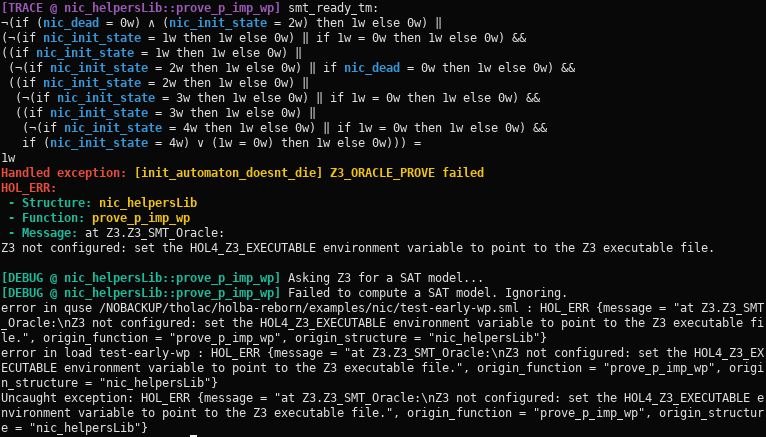
\includegraphics[width=\textwidth]{figures/loglib-ppexn-ppterm.png}
	\centering
	\caption{Extract of a script output, featuring \textit{trace} and \textit{debug} information from \textit{logLib} (Section \ref{loglib}), and an exception printed using the exception pretty-printer (Section \ref{pp_exn}). The original exception can be seen in white at the bottom of the image.}
	\label{loglib-ppexn-ppterm}
\end{figure}

\subsection{SML exception pretty-printer} \label{pp_exn}

As can be seen in Figure \ref{loglib-ppexn-ppterm}, default printing of HOL4 exceptions is not really easy to decipher. The is due to the fact that HOL4 has been designed as an \textbf{interactive} theorem prover to be used with \textit{Emacs}, which provides some layout and pretty-printing features. Therefore, a small pretty-printing library for SML exceptions has been implemented, called \textit{pretty\_exnLib}. It provides only two analogous functions that, given an exception as parameter, pretty-print the exception and return it unchanged. Listing \ref{pretty_exnLib_sig} presents the signature of the library, and Listing \ref{pretty_exnLib_usage} shows how it is used.

\begin{lstlisting}[
    language=Caml,
    backgroundcolor=\color{codebackcolour},
    commentstyle=\color{codegreen},
    keywordstyle=\color{magenta},
    stringstyle=\color{codepurple},
    label=pretty_exnLib_sig,caption={Signature of the \textit{pretty\_exnLib} library.},
    frame=tb,basicstyle=\footnotesize\ttfamily,
    float,floatplacement=H]
signature pretty_exnLib =
sig
  val pp_exn: exn -> exn
  val pp_exn_s: string -> exn -> exn
end
\end{lstlisting}


\begin{lstlisting}[
    language=Caml,
    backgroundcolor=\color{codebackcolour},
    commentstyle=\color{codegreen},
    keywordstyle=\color{magenta},
    stringstyle=\color{codepurple},
    label=pretty_exnLib_usage,caption={Typical usage of the \textit{pretty\_exnLib} library.},
    frame=tb,basicstyle=\footnotesize\ttfamily,
    float,floatplacement=H]
(* some code  that can raise ... *)
handle e => raise pp_exn e;

(* or *)
handle e => raise pp_exn "Failed to perform A, check that B." e;
\end{lstlisting}


\section{Best practices for a complex platform} \label{best-practices-complex-platform}

When building complex systems, special care should be taken in order to ensure that it grows in good conditions. Despite providing the best capabilities, a system with poor usability will encounter a slow adoption, as shown in the previous section. But when a system gets used by an increasing number of users, a different working organization is needed. This section will first briefly introduce a critical concept that should be mastered for the successful growth of a software platform. Then, we will study the \gls{CI} system that has been set up for HolBA.

\subsection{Developing simple interfaces}

% Make sense for contract verification library

In 1995, the Gang of Four published a book about design patterns for software design \cite{gamma_design_1995}. ``Program to an interface, not an implementation.'' is a key concept presented among the patterns. Since then, this sentence is considered as one of the most important design principles in software development.

This section doesn't intend to give a thorough explanation of the concept. However, some key insights shall be provided:

\begin{itemize}
    \item An interface is a contract between a system (such as a function, a library, a platform) and its users. This contract states the behavior and guarantees that this system offers via its public components. It defines the interactions between the component, the system, and the user. But most importantly, the contract leaves out the implementation. An interface builds an abstraction over the implementation. Using explicit contracts is particularly useful when performing contract-based verification, as it can simplify reasoning about components and allow building a more resilient system.
    \item Libraries provide features, which sometimes have a very complex implementation. This is particularly true for trustworthy binary code analysis. Building interfaces helps to abstract away complex implementations and helps to compose systems together.
    \item Programming to an interface instead of an implementation makes the code more resilient to changes. Indeed, if an implementation must be changed in order to provide more features, fix critical bugs or deliver more performance, codes that are not aware of the implementation will not need to be modified.
\end{itemize}

%\subsection{Using a Git workflow suitable for teams}
% * merge often
% what else?

\subsection{Continuous Integration: tests and static analysis}

\acrfull{CI} is a development practice where developers of a project \textit{integrate} frequently their code and changes into a single shared source repository, hence the name of this practice. Each integration of any change into the shared repository should be automatically verified by automated builds and a full set of automated tests. This allows to immediately see if changes to the source repository break a feature or introduce a regression, thus allowing to fix it immediately. Since this practice imposes to run a whole battery of tests for each and every change, even the smallest one, automation is key. \cite{martin_fowler_continuous_nodate} gives a detailed introduction to this practice.

A CI system has been added to the HolBA repository, and its practices are being adopted by the research team. For each change, the CI system recompiles the whole platform from scratch and runs all the tests and executes a set of example scripts. Additionally, the CI system also performs some static analysis of the source code in order to give developers some key insight of the state of the code. Since there are no support for SML or HOL4 in existing CI systems, new conventions have been adopted and scripts developed in order to define the test framework. Additionally, two static static analyzers have been implemented, showing respectively the \textit{cheats} used in the formal proofs and the ``\textit{TODO}'' comments indicating left work to be done \footnote{At the time of writing, this feature has not been added yet to the CI system because of time constraints. However, it is ready to be integrated.}.

\chapter{Conclusions}

\section{Discussion}

The goal of this paper was to perform experiments about the automation of formal verification of devices at the binary level. The NIC model of \cite{haglund_formal_2016} has served as a central theme throughout the work. Work in this thesis has been divided in practice into three parts, in addition to the learning process due to the very steep learning curve of HOL4:

\begin{enumerate}
    \item \textbf{Implementation of the NIC BIR model}: the formal model of the NIC of \cite{haglund_formal_2016} has been partially implemented as a BIR program, and BSL has been added to the HolBA platform in order to make this task more convenient.
    \item \textbf{Non proof-producing automatic contract verification library}: a user-friendly (adjective rarely used to describe HOL4), convenient and automatized library for contract verification have been implemented. This library brings HolBA one step closer to ``one-button solutions'' for performing software verification. It features a non proof-producing translation of BIR expressions to expressions that can be exported to SMT solvers, and an extension of HOL4's SMT library has been realized in order to add reasoning about BIR memories.
    \item \textbf{Formal proof of a BIR program on a HOL4 state}: a novel usage of BIR and method for transferring properties from BIR program to formal HOL4 specification has been carried out. Additionally, while not automated, the work needed in order to implement automatic HOL4 tactics has been clearly identified. Every automation work should be preceded by a manual implementation of the task, that this proof intends to be.
\end{enumerate}

Throughout this work, a strong focus has been placed on ease of use and user-friendliness with BSL, the pretty-printer, the implementation of new logging utilities, guidelines about error handling in SML and with HOL4, and a friendly exception printer. We strongly believe that user experience of such complex platforms are of primary importance because it can dramatically reduce time spent in debugging and the need of exhaustive documentation. Furthermore, it can give users the desire to keep using the platform. If it is decided to put more work in HolBA in order to make it a powerful binary analysis platform, the research team is advised to consider this aspect while expanding HolBA capabilities.

Some failed experiments have also been realized, including the DepGraph tool that revealed to not be adapted to its intended usage or which would have needed to much work for too few benefits (though DepGraph's design is future-proof and the tool can easily be extended later if new needs or novel ideas appear), and the former two implementation attempts of the NIC model using flowcharts or C which have been found to not be suitable for device models.

\section{Future work}

The topic of software verification, while being as old as Computer Science, still have a lot of work to be done and paths to be explored. This thesis opens some paths that could be considered by someone interested in the topic.

The pretty-printer implemented in this work is a small experiment only scratching the surface of what can be done in HOL4. Further work in this domain should follow the concrete needs that arise with extended usage of BIR. Current limitations and possible further work of the pretty-printer presented in this document include:

\begin{itemize}
    \item the generated output isn't parsable, which is against HOL4 conventions where every printed term should be parsable by the HOL4 quoting system. A solution to this problem would be to implement a theory introducing definitions for the new abbreviations. However, some liberties taken in the pretty-printer cannot be parsed: (a) the flat printing of nested binary expressions of the same state, because they would need variable arity functions which are not available in HOL4, and (b) \textbf{if-then-else} statements in the current representation.
    \item the pretty-printer doesn't use infix operators, feature widely employed in custom syntax used in some theories, like \textit{wordsTheory}. Infix syntax for binary operators can dramatically reduce the verbosity of expressions, and give a more familiar representation that \textit{could} be simpler to work with.
    \item the choice of colors could be reviewed in order to more closely follow HOL4 convention and usage. For example, BIR types are highlighted in the same color as free variables. While creating a very limited chance of ambiguities, users familiar with HOL4 conventions can be annoyed with this inconsistency.
\end{itemize}

The non proof-producing contract verification library implemented in this work can be really useful for prototyping, but it cannot be used for trustful verification. The limitations it suffers could be reasonably fast to overcome, and they should be fixed especially if HolBA were to become a strong binary analysis platform. Limitations include (a) the impossibility to compose contract in order to reason about longer functions, to compose functions or to prove properties on not loop-free programs, and (b) the obvious limitation of not being proof-producing. Work is ongoing at the time of writing about weak-correctness and contract composition, answering to (a). The main blocker of (b) is the absence of a proof-producing ways of using SMT solvers for proving contracts (Equation \ref{eval_pre_imp_eval_wp}). The proof of Chapter \ref{trustful-nic-analysis} and its SML implementation identify what automatic procedures should be added to HolBA in order to perform step (b) and progress towards proof-producing automatic verification.% Additionally, the signature of \texttt{prove\_contract} should be reworked in order to enable mixing it with proof-producing code, after both (a) and (b) are solved. For example, it should work with HOL4 definitions instead of raw terms.

% TODO: SMT: axioms for faster reasoning about memory + exponential problem

% Left out:
% - During binary verification, we work with ASM instead of clean C code. Therefore, pre-postconditions are harder to define. Hence, this one-button solution would need more support to easily define those expressions.
% - Automate PP proof: tactics that automatically add all the needed lemmas?

%%%%%%%%%%%%%%%%%%%%%%%%%%%%%%%%%%%%%%%%%%%%%%%%%%%%%%%%%%%%%%%%%%%%%%%%%%%%%%%%%%%%%%%%%%%%%

\printbibliography[heading=bibintoc]

\appendix

\chapter{DepGraph's design} \label{appendix_depgraph}
\vspace{-1cm}
\textit{This appendix briefly presents the design of DepGraph, the tool introduced in Chapter \ref{chapter-overview-nic}. While this experiment didn't reveal to be successful in order to get insights of the formal NIC model of \cite{haglund_formal_2016}, the tool still presents a powerful architecture and can be useful in order to generate documentation of \gls{SML} modules.}

DepGraph is a Python software that has been designed with modularity and extensibility in mind. The architecture is centered around a common data structure, the dependency graph, that is created by \textit{frontends}, mutated by \textit{middlewares} and exported by \textit{backends}. Figure \ref{depgraph-class-diagram} shows DepGraph's class diagram. Adding new frontends, middlewares or backends is as simple as adding one independent file and declare it the corresponding \textit{\_\_init\_\_.py}, and doesn't require to change any other code. Therefore, DepGraph allows easy creation of pipelines, that are a succession of one frontend, multiple middlewares and ended with one backend, and it can easily by extended to any need.

\begin{figure}[p]
	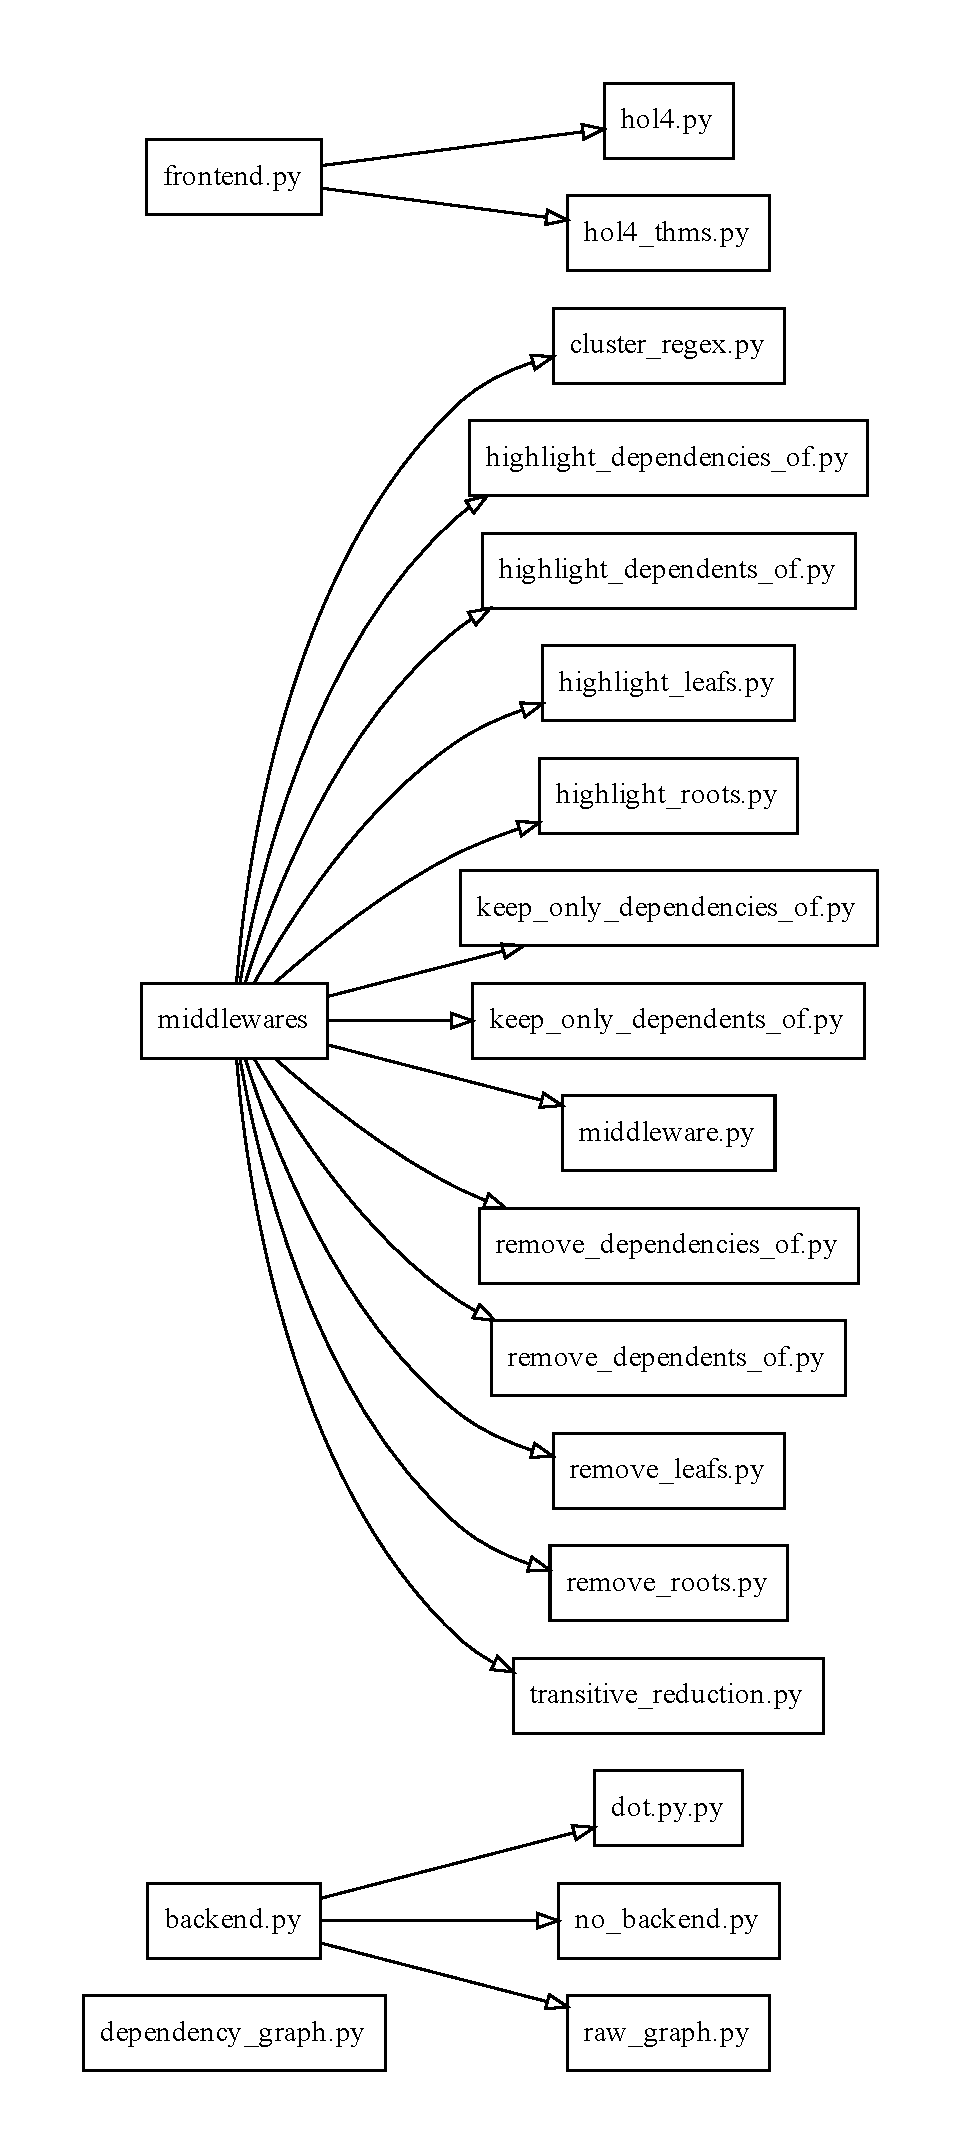
\includegraphics[height=16cm]{figures/depgraph-class-diagram.pdf}
	\centering
	\caption{DepGraph's class diagram, showing frontends, middlewares, and backends. The common intermediate representation, the dependency diagram, is implemented in \textit{dependency\_graph.py}.}
	\label{depgraph-class-diagram}
\end{figure}

%%%%%%%%%%%%%%%%%%%%%%%%%%%%%%%%%%%%%%%%%%%%%%%%%%%%%%%%%%%%%%%%%%%%%%%%

\tailmatter % back cover page

\end{document}
